\documentclass[journal]{IEEEtran}
\hyphenation{op-tical net-works semi-conduc-tor}
\setcounter{tocdepth}{2}

\usepackage{amssymb}
\usepackage{textcomp}
\usepackage{algorithm}
\usepackage{algorithmic}
\usepackage{fixltx2e}
\usepackage{url}
\usepackage{cite}
%\usepackage[margin=1in]{geometry}
\usepackage[latin1]{inputenc}
\usepackage{graphicx}
\usepackage{listings}
\usepackage{color}
\usepackage{xcolor}
\usepackage{paralist}
%\usepackage{caption}
%\usepackage{subcaption}


\usepackage{hyperref}
\hypersetup{
    colorlinks,
    citecolor=black,
    filecolor=black,
    linkcolor=black,
    urlcolor=black
}

\usepackage{tikz}
\usepackage{tikz-er2}
\usetikzlibrary{shapes,arrows}
\usetikzlibrary{positioning}
\usetikzlibrary{shadows}
\tikzstyle{every entity} = [top color=white, bottom color=blue!30,
                            draw=blue!50!black!100, drop shadow]
\tikzstyle{every weak entity} = [drop shadow={shadow xshift=.7ex,
                                 shadow yshift=-.7ex}]
\tikzstyle{every attribute} = [top color=white, bottom color=yellow!20,
                               draw=yellow, node distance=1cm, drop shadow]
\tikzstyle{every relationship} = [top color=white, bottom color=red!20,
                                  draw=red!50!black!100, drop shadow]
\tikzstyle{every isa} = [top color=white, bottom color=green!20,
                         draw=green!50!black!100, drop shadow]
\tikzstyle{decision} = [diamond, draw, fill=red!20,
    text width=4.5em, text badly centered, node distance=3cm, inner sep=0pt]
\tikzstyle{block} = [rectangle, draw, fill=blue!20,
    text width=5em, text centered, rounded corners, minimum height=4em]
\tikzstyle{edge} = [draw,line,-]
\tikzstyle{line} = [draw, -triangle 45]
\tikzstyle{cloud} = [draw, ellipse,fill=red!20, node distance=3cm,
    minimum height=2em]
\tikzstyle{dot} = [draw, circle, inner sep=1pt, fill=black]
\tikzstyle{db} = [draw,
  shape=cylinder,
  aspect=0.7,
  minimum height=2.5cm,
  minimum width=1.5cm,
  left color=yellow!30,
  right color=yellow!60,
  middle color=yellow!20, % Has to be called after left color and middle color
  outer sep=-0.5\pgflinewidth, % to make sure the ellipse does not draw over the lines
  shape border rotate=90
]


\definecolor{dkgreen}{rgb}{0,0.6,0}
\definecolor{gray}{rgb}{0.5,0.5,0.5}
\definecolor{mauve}{rgb}{0.58,0,0.82}
\lstset{ %
  language=SQL,                % the language of the code
  basicstyle=\scriptsize,           % the size of the fonts that are used for the code
  numbers=none,                   % where to put the line-numbers
  numberstyle=\tiny\color{gray},  % the style that is used for the line-numbers
  stepnumber=2,                   % the step between two line-numbers. If it's 1, each line 
                                  % will be numbered
  numbersep=5pt,                  % how far the line-numbers are from the code
  showspaces=false,               % show spaces adding particular underscores
  showstringspaces=false,         % underline spaces within strings
  showtabs=false,                 % show tabs within strings adding particular underscores
  rulecolor=\color{black},        % if not set, the frame-color may be changed on line-breaks within not-black text (e.g. comments (green here))
  tabsize=2,                      % sets default tabsize to 2 spaces
  breaklines=true,                % sets automatic line breaking
  breakatwhitespace=false,        % sets if automatic breaks should only happen at whitespace
                                  % also try caption instead of title
  keywordstyle=\color{blue},          % keyword style
  commentstyle=\color{dkgreen},       % comment style
  stringstyle=\color{mauve},         % string literal style
  escapeinside={\%*}{*)},            % if you want to add LaTeX within your code
  morekeywords={*,...}               % if you want to add more keywords to the set
}

\colorlet{punct}{red!60!black}
\definecolor{background}{HTML}{EEEEEE}
\definecolor{delim}{RGB}{20,105,176}
\colorlet{numb}{magenta!60!black}
\lstdefinelanguage{json}{
    basicstyle=\scriptsize\ttfamily,
    showstringspaces=false,
    breaklines=true,
    literate=
     *{0}{{{\color{numb}0}}}{1}
      {1}{{{\color{numb}1}}}{1}
      {2}{{{\color{numb}2}}}{1}
      {3}{{{\color{numb}3}}}{1}
      {4}{{{\color{numb}4}}}{1}
      {5}{{{\color{numb}5}}}{1}
      {6}{{{\color{numb}6}}}{1}
      {7}{{{\color{numb}7}}}{1}
      {8}{{{\color{numb}8}}}{1}
      {9}{{{\color{numb}9}}}{1}
      {:}{{{\color{punct}{:}}}}{1}
      {,}{{{\color{punct}{,}}}}{1}
      {\{}{{{\color{delim}{\{}}}}{1}
      {\}}{{{\color{delim}{\}}}}}{1}
      {[}{{{\color{delim}{[}}}}{1}
      {]}{{{\color{delim}{]}}}}{1},
}

% algorithm stuff
\newcommand{\sq}[0]{\textquotesingle}
\newcommand{\SWITCH}[1]{\textbf{switch}~#1 \\}
\newcommand{\CASE}[1]{~~~~\textbf{case}~#1 \\}


\newcommand{\pad}{\vbox to 20pt{}}
\newcommand{\bt}[1]{ \textbf{\texttt{#1}} }
\newcommand{\var}[1]{\texttt{#1}}
\newcommand{\term}[1]{\textit{#1}}

\newcommand{\schema}[0]{\term{/api/schema~}}
\newcommand{\metamodel}[0]{\term{/api/metamodel~}}
\newcommand{\sync}[0]{\term{/api/sync~}}
\newcommand{\create}[0]{\term{/api/create~}}

% vocab terms
\newcommand{\modts}[0]{\term{mod\_ts~}}


%-------------------------------------------------------
\begin{document}
\title{A Minimalist Data Access System\\ for Android Clients}
\author{Anthony Naddeo \\ Advisor: Sudarshan Chawathe}

\maketitle


\begin{abstract}
CRUD applications are those that enable users to create, read, update and delete
data from some specified data set, often a relational database. The
differences between CRUD applications lie primarily in the data that they
manage, not in features or expectations. We present a model for representing the
relationship between the standard CRUD operations and the data that is being
managed. With this model, it is possible to write a single CRUD application that
can be used to manage any set of data that uses a relational database. We define
a protocol that enables arbitrary amounts and types of clients to perform CRUD
operations on the same database. We also present a protocol for replicating
database instances across arbitrary DBMSs. These ideas have been combined into
one easily deployable system that can be used to create and maintain CRUD
applications without writing client source code.
\end{abstract}

\begin{IEEEkeywords}
Android, CRUD, meta model, database replication
\end{IEEEkeywords}

\IEEEpeerreviewmaketitle
\tableofcontents



%--------------------------------------------------------
\section{Introduction} \label{sec:intro}
%--------------------------------------------------------


The term CRUD refers to the four basic operations on persistent storage: create,
read, update and delete. Many CRUD focused applications implement their
persistence layers using relational databases. Of these applications, many
require multiple users to be able to perform CRUD operations on the same
database\footnote{give an example} from arbitrary client types (Android, Web
etc.). The data managed by CRUD applications varies greatly, but functionality
and user interfaces are largely the same across instances. For this reason,
there have been many frameworks that aid developers in creating their own CRUD
applications, but most of them require the programmer to write code (i.e. PHP or
Java) in order to generate entire applications that can be installed or placed
on a Web server; this quickly complicates an otherwise simple application. 

The use of a framework should be a categorically simpler experience than
building a CRUD application from scratch. Currently, the framework that best
meets this requirement is called Evolutility. Evolutility
is effective because the programmer only has to create XML configuration files
that describe UI forms that are generated at run time. This approach results in
a generic application that can be configured to display any type of data without
needing to edit the source. That being said, the project has some shortcomings,
particularly in its lack of native mobile application support (Android
specifically) and its dependency on proprietary Microsoft technology (as opposed
to open standards like Apache, PHP and MySQL). 

In this paper, we expand the generic CRUD application model described by
Giulieri\footnote{cite} to enable arbitrary client types and support mobile
clients by adding features like database replication for off line reading. This
project was originally an inventory application designed for Networkmaine, the
Internet service provider (ISP) for the public schools and libraries of Maine.


%--------------------------------------------------------
\subsection{Motivating Examples} \label{sec:motivation}
%--------------------------------------------------------

In this section, we provide examples that illustrate the initial constraints
 for this project.

%--------------------------------------------------------
\subsubsection{Mobile phones are often off line}  \label{sec:offline}

Libraries often cannot afford dedicated technical staff. When equipment breaks,
an employee of Networkmaine is likely to be dispatched to the site to install a
replacement. The equipment at libraries is commonly stored in the basements
where little-to-no wifi or mobile signal can reach. If the staff member does not
know which of the two router ports should provide the site with internet, then,
regardless of signal, they should be able to use their mobile device to retrieve
that information.



%--------------------------------------------------------
\subsubsection{Some users will only use browsers}  \label{sec:browser}

There are many network tools that are available exclusively through browsers at
Networkmaine. Mobile applications will have to coexist in the same system as Web
and desktop based applications.


%--------------------------------------------------------
\subsubsection{The database schema is likely to change over time}
\label{sec:change}

Most of the technical employees at Networkmaine are network engineers; very few
of them are even familiar with Android development. All application maintenance
will ultimately fall on the shoulders of someone who would rather being doing
something else. It is reasonable to assume that they might need to start
tracking other device types, or additional dates at some point in time. Changes
of this sort should not require recompilation of the application or any source
code modification.


%--------------------------------------------------------
\subsubsection{Entirely separate applications will eventually be needed}
\label{sec:deployable}

It is also reasonable to assume that Networkmaine may have a need to track
something entirely unrelated to networking devices (enrollment information
perhaps). Additional instances of CRUD applications should be easy to configure
and deploy.


%--------------------------------------------------------
\subsection{Overview}  \label{sec:overview}

% describe the structure of this project, what was used. The user should not be surprised by any of the following main sections after this section. He should expect a "Mirror method / Sync" section, "JSON ui form model" section, etc.

% explain server setup

% explain server side technologies

% explain android client setup
% explain android client dependencies 

% explain JSON stuff based on evolutility


We are interested in creating a generic CRUD system that shares a single database among arbitrary amounts (and types) of clients. In order to be effective, it must 
\begin{inparaenum}
\item be easier to use than creating a CRUD application,
\item allow off line reading on mobile clients,
\item have easily deployable instances for different databases and
\item never require source code modification for updates\footnote{Bugs in the source code will clearly require more traditional updates, but clients should adapt to the addition of tables or columns to the database.}.
\end{inparaenum}
In order to meet these requirements, we must have a way of replicating databases across arbitrary DBMS, isolate the parts of application instances that need to be customized (i.e. name and icon), and describe the UI enough for clients to display lists and forms that enable CRUD operations. Giulieri summarized his efforts well in his entry into the Code Generator 2008 Competition\cite{giulieri_minimalist_2011}
\begin{quotation}
``We argue that the key concept here is the representation of UI Metadata and that with a proper set of fundamental UI widgets, most CRUD applications can be effectively designed without hand coding.''
\end{quotation}
We use Giulieri's Evolutility\cite{giulieri_evolutility_????} project as a starting point. Evolutility consists of various .aspx pages and dlls that need to be copied to a Web server, along with some SQL scripts that need to be run to create tables that store meta data. Once the initial configuration is done, an XML file can be created that specifies the relation between fields on forms and entities in the database. The XML file format is specified in his Code Generator 2008 Competition entry\cite{giulieri_minimalist_2011}. 

In our project, \texttt{Coexist}, we use different technologies. One of
the goals of our project is to be more accessible than Evolutility by using open
and free (as in money) software when possible; consequently, Coexist uses a
typical LAMP stack for the server, instead of ASP.NET and SQL Server.

We use JSON instead of XML for the model. The framework is designed in such a
way that XML support can be added in the future, but JSON will be supported from
the start. The same XML data can usually be represented with fewer bytes in JSON
and can also be easier to hand edit. In addition, we already had experience with
Google's Gson library and there were no significant reasons to prefer XML.

As mentioned, the server side code is written in PHP and is designed as an API.
The API exposes four resources to clients, each one fulfilling a particular
responsibility.

\begin{itemize}
\item \textbf{/api/sync}: Provides clients with the rows of the database that they are missing based on timestamp information.
\item \textbf{/api/schema}: Sends SQL to the client that creates the necessary tables on its local database. The DBMS type must be supplied in requests (i.e. SQLite).
\item \textbf{/api/crud}: Sends the JSON model to the client so that it can create UI forms.
\item \textbf{/api/create}: Creates or updates rows on the server. These rows are retrievable through calls to /api/sync.
\end{itemize}

An Android client implementation has also been provided. It uses the recommended
Java based tools from Google, as well as the Android Support library and the
ActionbarSherlock library\cite{wharton_actionbarsherlock_????} for backwards
compatibility. At the moment, these dependencies are required in order to
produce a viable client, though this may change as older versions of Android are
aged out. Using third party libraries can be risky at times, but even Google
seems to have made use of ActionbarSherlock in their own
applications\cite{google_baseactivity.java_????}.

For the database replication we require a server side DBMS that supports
triggers (MySQL, PostgreSQL, etc.). The replication utilizes timestamps to
synchronize clients. Since one of our goals is full off line readability,
Coexist is most suitable for smaller sized databases (the entire database will
be replicated on the client's internal storage).


%--------------------------------------------------------
\subsection{Related Works} \label{sec:related}
% talk about what people are doing to solve this at the moment

Evolutility\cite{giulieri_evolutility_????} was by far the closest match to what
we were trying to do, but before finding it there were several other projects
that were encountered and rejected for various reasons. Android Crud Code
Generator (ACCG)\cite{popovski_android-crud-code-generator_????} and
Phreeze\cite{hinkle_phreeze_????} are representative of the kinds of projects
that we were finding. The first is targeted at Android and the second is PHP,
but both of them aim to make the CRUD experience simpler. Phreeze is a polished
application, but it requires users to write code during the "development"
process, which violated our requirements. ACCG took a different approach. It
generates all of the Java code that would be needed when making a CRUD
application. This is similar from a user perspective, but we ultimately want to
have one code base that never has to be modified; not to mention, it is strictly
local storage. OpenMobster's CRUD
Tutorial\cite{openmobster_mobilizehibernate_????} introduced us to the Hibernate
framework\cite{jboss_community_hibernate_????} for object relational mapping.
This is a mature framework that enables transparent persistence of Java objects.
This violates our goal of minimizing requirements, as well as requiring code to
be written; non the less, it is an impressive and interesting framework. 


%% fix formatting for its new context
In the realm of database replication, we considered an interesting solution from
fyreCloud's Amsler project. It was designed with Android in mind, attempting to
mediate the MySQL replication protocol to make it compatible with
SQLite\cite{fyrecloud_solutions_fyrecloud_????}. The actions of the Amsler
project can be summarized as follows.

\begin{enumerate}
\item Configure the MySQL back end for data replication as described by the MySQL manual. 
\item Use TCP/IP connections to continuously push changes to the client in the form of MySQL commands.
\item Use a lexer and parser to map the incoming MySQL queries to valid SQLite queries. 
\end{enumerate}

Step 3 was troublesome; the syntax of different SQL implementations has many
subtle differences. The idea of having a limited set of queries (dictated by the
Amsler project's progress) that we could use on the server was an unnecessary
burden.


%% fix formatting
The popular client authentication method today is the OAuth
library\cite{_oauth_????} used by Facebook, Twitter and LinkedIn to name a few.
The idea is to use authentication tokens in place of passwords so that third
party applications can access someone's information by making requests with
tokens instead of passwords. For the purposes of Networkmaine, there will be no
third party plug in service and all users access the same information over SSL.
Storing local password hashes or requesting passwords per transaction (depending
on us

%--------------------------------------------------------
\subsection{Outline of Paper} \label{sec:outline}


The remainder of this paper is organized as follows. Section~\ref{sec:xml}
reviews the XML-based meta-model presented by Giulieri and
Section~\ref{sec:json} introduces the JSON version of it used by Coexist.
Section~\ref{sec:db} describes the protocol used to enable database replication
across arbitrary DBMSs. In Section~\ref{sec:api}, we take a closer look at the
structure of the Web server and API, and what interaction with clients will look
like. Section~\ref{sec:deployment} examines the system as a whole from the end
user's perspective. It will also detail the work involved with customizing an
Coexist instance and deploying it. We conclude in Section~\ref{sec:conclusion}.




%--------------------------------------------------------
\section{The Server and API} \label{sec:api}
%--------------------------------------------------------

In the Coexist client-server model, the clients communicate with the server
through an HTTP based API. This section will specify the details of the
communication between the server and clients, starting with the declaration of
necessary API methods in Section~\ref{sec:api_methods}.


%--------------------------------------------------------
\subsection{API Methods}  \label{sec:api_methods}

% declaring the api methods, not implementing


% maybe introduce the data replication stuff before this point. 
The API can be designed by taking the client's needs into
consideration. In Coexist, every client has a local copy of their central
database, so every client must be able to
\begin{inparaenum}
\item create their local database,
\item present the user with forms for data entry,
\item request missing information from the server, and
\item add information to the server.
\end{inparaenum}
Since the clients will be communicating with the API over HTTP, the server-side
methods will be accessed through URLs of the form
\mbox{\texttt{http://domain.com/api/name}}, where \texttt{name} will be
the name of a particular resource. These client needs translate roughly into the
following server side methods.

%--------------------------------------------------------
\subsubsection{/api/schema}  \label{sec:api_schema}
This resource will return the information that the clients need in order to
build their local databases and replicate the server's database.

%--------------------------------------------------------
\subsubsection{/api/metamodel}  \label{sec:api_metamodel}
This resource will return the information that clients need in order to present
and gather information to and from users.

%--------------------------------------------------------
\subsubsection{/api/sync}  \label{sec:api_sync}
This resource will provide clients with all of the database rows that are
currently absent from their local databases.

%--------------------------------------------------------
\subsubsection{/api/create}  \label{sec:api_create}
Clients will send requests to create rows on the central server to this
resource.

Figure~\ref{fig:client_states} is a state based diagram that shows how clients can
learn how to create their local databases, display information to users,
synchronize themselves and create new information on the server. 

\begin{figure}[h!]
\centering
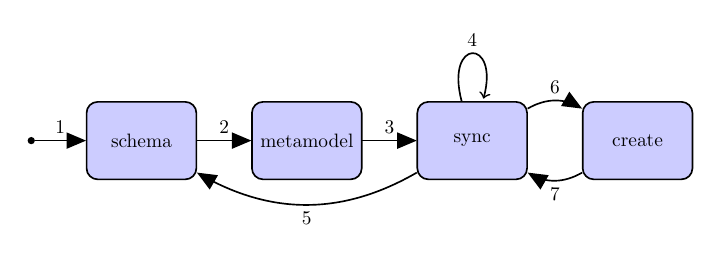
\begin{tikzpicture}[node distance = 3cm, semithick, auto, scale=.7, every node/.style={transform shape}]
  % Place nodes

  \node [dot] (start) {};
  \node [block, right of=start, node distance=2cm] (s1) {schema};
  \node [block, right of=s1] (s2) {metamodel};
  \node [block, right of=s2] (s3) {sync};
  \node [block, right of=s3] (s4) {create};
 
  \path [line] (start) -- node {1} (s1) ;
  \path [line] (s1) -- node {2} (s2);
  \path [line] (s2) -- node {3} (s3);

  \path (s3) edge [loop above] node {4} (s3);
  \path (s3) edge [line,bend left] node {5} (s1);

  \path (s3) edge [line, bend left] node {6} (s4);
  \path (s4) edge [line, bend left] node {7} (s3);

\end{tikzpicture}
\caption{A state based representation of Coexist clients. Using only the four
API methods provided, a client can build its local database, learn how to
display it, sync itself and create new information on the server.}
\label{fig:client_states}
\end{figure}

Clients start out on edge 1 without any information. By the time they reach edge
3, they have everything they need in order to build local databases for
replicating the server, as well as metadata relating to the display of the
database contents. The next step is a call to \texttt{/api/sync} to pull down
missing rows from the server (which will be all rows on the first run).
Consecutive calls allow clients to stay in sync while other clients make
changes to the database. Every time a row is created on the database through
a call to \texttt{/api/create}, it resynchronizes itself and imports the newly
created rows into its local database. At this point it can take edge 5 to
restart the entire process, allowing it to respond to changes in the server's
database schema.

So far, we have a rough idea of what clients need and what the server
must provide them, but not enough to know exactly how to implement these methods
on the server. For example, we have questions about
\begin{inparaenum}
\item\label{enum:data} what the data exchange format between clients and the server will be, 
\item\label{enum:sync} how to synchronize data, and
\item\label{enum:meta} how to tell clients to display the synced data to users. 
\end{inparaenum}

The next section will answer questions \ref{enum:data} and
\ref{enum:sync} by introducing a simple method of communication that allows
clients to maintain the integrity of their local databases, as well as a
stateless synchronization protocol for relational databases that can be
implemented in pure SQL. In Section~\ref{sec:metamodel}, we answer
question~\ref{enum:meta} by defining a JSON based metamodel that contains all of
the information necessary for clients to display and collect data from users.
Finally, in Section~\ref{sec:deployment}, the build process will be described.
%Finally, in Section~\ref{sec:api_imp}, these four API methods are revisited and
%fully implemented.



%
%%-------------------------------------------------------
%\subsection{Client-Server Communication}
%
%%Many mobile applications are supplemented by a local database (typically
%%SQLite). Some applications are stand alone and use these databases primarily as
%%persistent storage; the Networkmaine inventory application uses its local
%%database to interface with the remote back end MySQL server that it depends
%%heavily on. There were three methods for this interfacing that represent
%%different degrees of caching, from none, to selective, to complete.
%
%
%%Before deciding upon a
%
%This section will explore some of the methods that the client can use to
%interface with the server, their advantages and disadvantages, and explain why
%the method labeled as the \textit{mirror method} is the appropriate choice. The
%following subsections will give details on the implementation of this method and
%its implications on the database schema; particularly, how normalized it should
%be and how to handle deletions. In all diagrams in this section, the arrows
%indicate the flow of data and the labels indicate the actions that cause them.
%
%
%%-------------------------------------------------------
%\subsubsection{Window method}
%
%In the window method, the data that a user sees at any given time is a window
%into the back end server; all of the data came from the server and none of it is
%going to persist beyond this screen. The major advantage to this method is its
%ease of implementation. This would be a suitable fit for a small weather
%application; in fact, it is the approach that my own weather application ,
%QtWeather, uses.  
%
%%TODO add some more analysis details
%
%\begin{figure}[h!]
%\centering
%\begin{tikzpicture}[node distance = 2cm, auto, scale=.7, every node/.style={transform shape}]
%  % Place nodes
%  \node [block] (client) {client};
%  \node [block, right of=client, node distance=5cm] (server) {server};
%  % Draw edges
%  \path [line] (server.165) -- node [above] {query} (client.15);
%  \path [line] (client.345) -- node [below] {udpate} (server.195);
%\end{tikzpicture}
%\caption{Window method}
%\label{fig:window}
%\end{figure}
%
%
%%-------------------------------------------------------
%\subsubsection{Cache method}
%
%Treating the client as a window requires that we don't have large amounts of
%data constantly being retrieved from the server. If this is not the case, then
%we may want to identify some data (or queries) that are commonly used in order
%to cache (and optionally sync) on the client's local database. This would be
%suitable for a mobile social networking client. Take a typical Facebook
%application for example; it would be advantageous to cache a users top five
%commonly used groups as well as their friend list because this information is
%supposedly accessed often and is relatively static. In contrast, caching the
%Facebook news feed would probably result in a lot of wasted space because of how
%fast it changes and how rarely old news feed entries are viewed. 
%
%
%
%\begin{figure}[h!]
%\centering
%\begin{tikzpicture}[node distance = 2cm, auto, scale=.7, every node/.style={transform shape}]
%  % Place nodes
%  \node [block] (client) {client};
%  \node [block, right of=client, node distance=5cm] (server) {server};
%  \node [db, below of=client, node distance=4cm, align=center] (database) {local \\ database};
%
%  % Draw edges
%  % Need to align in order to line break
%  \path [line] (server.165) -- node [above, align=center] {query \\ un-cachable data} (client.15);
%  \path [line] (client.345) -- node [below] {update} (server.195);
%  \path [line] (server) |- node {sync cache} (database);
%  \path [line] (database) -- node [align=left] {query frequent \\ and static data} (client);
%\end{tikzpicture}
%\caption{Cache method}
%\label{fig:cache}
%\end{figure}
%
%
%%-------------------------------------------------------
%\subsubsection{Mirror method}
%The window method has the client retrieve all data from the server all of the
%time, the cache method identifies some useful data to store and then caches it
%locally; the mirror method is the next natural step in this progression: cache
%the entire database. There are some immediate concerns with this approach, most
%prominent of which concerns the size of the database potentially being much
%larger than the what we can reasonably expect to store on the client. The
%advantages to this method are faster query times and less reliance on the
%network. In fact, this is the only method that would enable a fully readable
%database off line.
%
%\begin{figure}[h!]
%\centering
%\begin{tikzpicture}[node distance = 2cm, auto, scale=.7, every node/.style={transform shape}]
%  % Place nodes
%  \node [block] (client) {client};
%  \node [block, right of=client, node distance=5cm] (server) {server};
%  \node [db, below of=client, node distance=4cm, align=center] (database) {local \\ database};
%
%  % Draw edges
%  % Need to align in order to line break
%  \path [line] (client) -- node {udpate} (server);
%  \path [line] (server) |- node {mirror} (database);
%  \path [line] (database) -- node [align=left] {query} (client);
%\end{tikzpicture}
%\caption{Mirror method}
%\label{fig:mirror}
%\end{figure}
%
%The Networkmaine inventory database contains information for approximately six
%thousand devices, location, purchase order and rma information for batches of
%devices; the size of the MySQL database dump is 1.5 megabytes. In addition, the
%database will not grow quickly. The size of the database makes the mirror method
%very attractive: if Networkmaine added two thousand units a year to its
%deployment then in twenty years the size of the database would be no less than
%12 megabytes; still reasonable to store on the mobile clients we see available
%today (probably more so on the mobile clients in twenty years, if we still use
%them). Realistically, there won't be more than a few hundred devices added to
%the inventory each year, at most. It is for these reasons that the mirror method
%is preferable for this project. 
%
%
%
%
%%-------------------------------------------------------
%\subsection{Implementation}
%
%Many database systems support mirroring, or data replication. The driving factor
%in this technology seems to be data availability: always having a slave database
%server that can assume the primary role in the event that something goes
%wrong\cite{microsoft_database_????}. The issue here is that we don't have much
%control over the development environment; the server side database is MySQL
%because that is what the staff is familiar with and the client side database is
%SQLite because that is what Android supports. While MySQL does support data
%replication to MySQL slave servers, it certainly does not support replication to
%arbitrary alternative DBMS\cite{mySQL_mySQL_????}.
%
%%That does not mean it is impossible. We considered an interesting solution from
%%fyreCloud's Amsler project. It was designed with Android in mind, attempting to
%%mediate the MySQL replication protocol to make it compatible with
%%SQLite\cite{fyrecloud_solutions_fyrecloud_????}. The actions of the Amsler
%%project can be summarized as follows.
%%
%%\begin{enumerate}
%%\item Configure the MySQL back end for data replication as described by the MySQL manual. 
%%\item Use TCP/IP connections to continuously push changes to the client in the form of MySQL commands.
%%\item Use a lexer and parser to map the incoming MySQL queries to valid SQLite queries. 
%%\end{enumerate}
%%
%%Step 3 was troublesome; the syntax of different SQL implementations has many
%%subtle differences. The idea of having a limited set of queries (dictated by the
%%Amsler project's progress) that we could use on the server was too much to bear.
%
%A simpler approach to this problem involved the addition of \textit{metacolumns}
%to the original schema; or columns defined in a SQL table that do not
%traditionally relate to the other columns in that table, but instead are used
%for some application level purpose. The most important of these metacolumns is
%the \texttt{mod\_ts} (modification timestamp) column. Let's take a simple
%relation \hbox{\texttt{Student(id, name, year)}} and examine how it can be
%synchronized across multiple instances without using any DBMS specific features.
%In this example, both the client and server tables are initialized to the table
%in Figure~\ref{fig:student_init}. 
%
%
%\begin{figure}[h!]
%\center
%\begin{tabular}{ l  l  l  l }
%id  & name      & year  & \textit{mod\_ts} \\
%\hline
%1   & Anthony   & 4     & \textit{0}        \\
%2   & Lucas     & 3     & \textit{0}        \\
%3   & Steven    & 3     & \textit{0}        \\
%\end{tabular}
%\caption{Initial state of the \texttt{Student} table.}
%\label{fig:student_init}
%\end{figure}
%
%As implied, the \texttt{mod\_ts} metacolumn will be updated with the time of the
%transaction. For the purpose of readability, we represent this timestamp as the
%number of seconds since the creation of the table. 
%
%Now lets update the server from one of the many possible client applications. 
%
%
%\begin{figure}[h!]
%\begin{lstlisting}[language=sql]
%BEGIN TRANSACTION;
%INSERT INTO Student(name,year) VALUES(Ryan, 4);
%UPDATE Student SET year=4 WHERE name='Lucas';
%COMMIT;
%\end{lstlisting}
%\caption{Transaction on the server.}
%\label{fig:student_transaction1}
%\end{figure}
%
%It is worth mentioning now that the following trigger must exist on the server
%database for \texttt{INSERT}, \texttt{UPDATE} and \texttt{REPLACE} (but not
%necessarily for \texttt{DELETE}, explained in section \ref{sec:schema}).
%
%
%\begin{figure}[h!]
%\begin{lstlisting}[language=sql]
%CREATE TRIGGER mod_ts AFTER INSERT ON Student
%  FOR EACH ROW SET mod_ts = NOW();
%\end{lstlisting}
%\caption{Trigger for modification timestamps.}
%\label{fig:student_trigger}
%\end{figure}
%
%The transaction of figure~\ref{fig:student_transaction1} will leave the server
%in the following state.
%
%\begin{figure}[h!]
%\center
%\begin{tabular}{ l  l  l  l }
%id  & name      & year  & \textit{mod\_ts} \\
%\hline
%1   & Anthony   & 4     & \textit{0}        \\
%2   & Lucas     & 4     & \textit{10}        \\
%3   & Steven    & 3     & \textit{0}        \\
%4   & Ryan      & 4     & \textit{10}        \\
%\end{tabular}
%\caption{Server state after transaction of figure \ref{fig:student_transaction1}.}
%\label{fig:student_update}
%\end{figure}
%
%Currently all clients are still in the state of figure~\ref{fig:student_update}
%and need to be synchronized with the server; this is a multi-part process,
%central to which is the client side query in figure~\ref{fig:student_change}. 
%
%\begin{figure}[h!]
%\begin{lstlisting}
%SELECT max(mod_ts) FROM Student;
%\end{lstlisting}
%\caption{Find the most recent local change.}
%\label{fig:student_change}
%\end{figure}
%
%In our case (and in many cases), the client communicates with the server
%database through a RESTful API. One such function provided by this API is
%$getChanges(table,~ts)$, where $table$ is the name of a table and $ts$ is a
%timestamp. In our running example, all clients would have to send a call to
%$getChanges(~Student,~0)$, where $0$ was returned from the query of
%figure~\ref{fig:student_change}. The server will respond to the client by
%returning all rows of the Student table where $mod\_ts > 0$, enabling the client
%to insert or replace them locally. If the most recent change on the client side
%is the same as the most recent change on the server then they are in
%sync\footnote{Recall from figure~\ref{fig:mirror} that the client never modifies
%its local database, it only requests synchronization from the server.}.
%
%
%
%%--------------------------------------------------------
%\subsection{Handling Deletes}  \label{sec:}
%
%Section~\ref{sec:api} introduced the Mirror Method and discussed an
%implementation that would allow stateless synchronization with multiple clients
%using pure SQL. An issue arose when trying to incorporate SQL \texttt{DELETE}s into the
%system: because server side changes were synchronized with clients using
%\mbox{modification} timestamps, deleted rows would not be propagated to clients. In
%order to support the DELETE operation and preserve the synchronization, an
%additional metacolumn was added: \textit{deleted}.  This metacolumn tells the
%Coexist clients to hide rows from the interface, giving the illusion of
%deletion. This modification would turn Figure~\ref{fig:student_update} into
%Figure~\ref{fig:new_deleted}.
%
%\begin{figure}[h!]
%\center
%\begin{tabular}{ l  l  l  l  l}
%id  & name      & year  & \textit{mod\_ts} & \textit{deleted} \\ 
%\hline
%1   & Anthony   & 4     & \textit{0}   & \textit{0}     \\
%2   & Lucas     & 4     & \textit{10}   & \textit{0}     \\
%3   & Steven    & 3     & \textit{0}   & \textit{1}     \\
%4   & Ryan      & 4     & \textit{10}   & \textit{0}     \\
%\end{tabular}
%\caption{Introducing the \textit{deleted} metacolumn.}
%\label{fig:new_deleted}
%\end{figure}
%
%In this example, \texttt{Steven} would have been marked as deleted from the
%database and hidden from the user interface. Because the change happens in a
%column, it can be propagated out to the server and ultimately the other clients
%without having to change the modification-timestamp-based approach decided in
%Section~\ref{sec:api}.
%
%Unfortunately, two additional problems arose from this fix: 
%\begin{inparaenum}
%\item The deleted rows build up on the server.
%\item The primary keys are still occupied. 
%\end{inparaenum}
%The buildup of rows can be remedied by periodically deleting all rows marked as
%deleted and triggering resynchronizations on the clients. This would cause them
%to delete their local databases and download all missing rows (which would no
%longer include deleted rows). This is only necessary if the deleted rows start
%to occupy a significant amount of space.
%
%The primary key issue was more serious. In Figure~\ref{fig:new_deleted}, clients
%would no longer be able to add a \texttt{Steven} to the database after marking
%him as deleted, nor could they modify the row to un-delete him (assuming
%\texttt{name} is a primary key). The solution involved a small expansion of the
%API specification: the addition of a \texttt{replace} parameter to all requests
%made to \texttt{/api/create/}\footnote{Recall that this is the API method used
%for creating rows on the server.} from clients. Figure~\ref{fig:create} depicts
%  the actions of the API when receiving requests to \texttt{/api/create/}.
%
%
%\begin{figure}[h!]
%\centering
%\begin{tikzpicture}[node distance = 3cm, auto, scale=.7, every node/.style={transform shape} ]
%  % Place nodes
%  \node [block] (request) {Request to /api/create/};
%  \node [decision, below of=request] (isconflict) {Key violation?};
%  
%  \node [block, left of=isconflict] (create) {Create the row.};
%  \node [decision, right of=isconflict] (nocreate) {Does replace=1?};
% 
%  \node [block, below of=create] (ok) {\textbf{200 OK}}; 
%
%  \node [dot, below of=nocreate] (nocreateDOT) {};
%
%  \node [block, left of=nocreateDOT] (replace) {Replace it};
%  \node [decision, below of=replace] (isreplace) {Does deleted=1};
%
%  \node [block, left of=isreplace] (error) {\textbf{409 Conflict}};
%
%  % Draw edges
%  \path [line] (request) -- (isconflict);
%  \path [line] (isconflict) -- node [above] {no} (create);
%  \path [line] (isconflict) -- node [above] {yes} (nocreate);
%  \path [line] (create) -- (ok);
%
%  \path [edge] (nocreate) -- (nocreateDOT);
%  \path [line] (nocreateDOT) -- node [above] {yes} (replace);
%  \path [line] (replace) -- (ok);
%
%  \path [line] (nocreateDOT) |- node [right] {no} (isreplace);
%  \path [line] (isreplace) -- node [right] {yes} (replace);
%
%  \path [line] (isreplace) -- node [above] {no} (error);
%
%\end{tikzpicture}
%\caption{API process for row creation.}
%\label{fig:create}
%\end{figure}
%
%The flow chart starts with ``Request to /api/create/'', which is a request
%to create a row on the server from a client. If there is no key constraint
%violation, then the row is created and the server responds with a \texttt{200
%OK}. If there is a violation then the server checks to see if the request's
%\texttt{replace} parameter is set to \texttt{1}. If it is then the conflicting
%row can be replaced without worry and the server responds with a \texttt{200
%OK}.  If not then the server checks to see if the conflicting row is marked as
%deleted. If it is, then the conflicting row can be replaced and the server
%responds with a \texttt{200 OK}. If not, then the server responds with a
%\texttt{409 CONFLICT} and the row is not created. At this point, the client has
%enough information to ask the user if they wish to replace (or update) the
%conflicting row on the server and potentially resend the request with
%\texttt{replace=1}. 
% 
%This solution reduces the functional burden of the deleted rows, enables SQL
%\texttt{UPDATE} functionality, is completely representable with pure SQL, and
%requires no significant changes to the existing API. 
%
%
%
%
%%--------------------------------------------------------
%\subsection{Database Replication} \label{sec:db}
%
%
%It is important to ensure that the client can never update the server if the
%client is out of sync, and the client must always have a way of re-syncing
%itself.  This can be achieved with two simple API functions, \texttt{/api/sync}
%and \texttt{/api/schema}; where one function requests missing information and
%another requests schema information. This design accounts for the database
%schema being upgraded on the server, and clients attempting to make changes to
%the database server when out of sync. Figure~\ref{fig:protocol} depicts the
%network dialog between a client and server where the client attempts to sync
%itself when it is using and old version of the database. 
%
%
%
%
%\begin{figure}[h!]
%\centering
%\begin{tikzpicture}[node distance = 2cm, auto, scale=.7, every node/.style={transform shape}]
%  % Place nodes
%  \node [block] (client) {client};
%  \node [block, right of=client, node distance=6cm] (server) {server};
%  
%  \node [dot, below of=client, node distance=2.5cm, label=180:1] (c1) {};
%  \node [dot, below of=server, node distance=2.5cm] (s1) {};
%  \path [line] (c1) -- node [above, align=left] {
%    \tt\textbf{GET /api/sync} \\ 
%    \tt version:1 \\ 
%    \tt tables:[t1,t2] \\ 
%    \tt mod\_ts:[33,12]}   (s1);
%  \path [edge] (client) -- (c1);
%  \path [edge] (server) -- (s1);
%
%  \node [dot, below of=c1, node distance=1cm, label=180:2] (c2) {};
%  \node [dot, below of=s1, node distance=1cm] (s2) {};
%  \path [line] (s2) -- node [above] {\tt\textbf{409 CONFLICT}} (c2);
%  \path [edge] (c2) -- (c1);
%  \path [edge] (s2) -- (s1);
%
%  \node [dot, below of=c2, node distance=1.5cm, label=180:3] (c3) {};
%  \node [dot, below of=s2, node distance=1.5cm] (s3) {};
%  \path [line] (c3) -- node [above, align=left] {
%    \tt\textbf{GET /api/schema} \\ 
%    \tt db:SQLite            } (s3);
%  \path [edge] (c2) -- (c3);
%  \path [edge] (s2) -- (s3);
%
%  \node [dot, below of=c3, node distance=2cm, label=180:4] (c4) {};
%  \node [dot, below of=s3, node distance=2cm] (s4) {};
%  \path [line] (s4) -- node [above, align=left] {
%    \tt\textbf{200 OK} \\
%    \tt\{version:2 \\
%    \tt~SQL:[CREATE TABLE...]\} } (c4);
%  \path [edge] (c3) -- (c4);
%  \path [edge] (s3) -- (s4);
%    
%  \node [dot, below of=c4, node distance=2cm, label=180:5] (c5) {};
%  \node [dot, below of=s4, node distance=2cm] (s5) {};
%  \path [line] (c5) -- node [above, align=left] {
%    \tt\textbf{GET /api/sync} \\ 
%    \tt version:2 \\ 
%    \tt tables:[t1,t2,t3] \\ 
%    \tt mod\_ts:[0,0,0]}   (s5);
%
%  \path [edge] (c5) -- (c4);
%  \path [edge] (s4) -- (s5);
%
%
%  \node [dot, below of=c5, node distance=2cm, label=180:6] (c6) {};
%  \node [dot, below of=s5, node distance=2cm] (s6) {};
%  \path [line] (s6) -- node [above, align=left] {
%    \tt\textbf{200 OK} \\
%    \tt \{t1:[(..),(..)] \\
%    \tt~t2:[] \\
%    \tt~t3:[] \}} (c6);
%  \path [edge] (c6) -- (c5);
%  \path [edge] (s6) -- (s5);
%
%\end{tikzpicture}
%\caption{Synchronization protocol}
%\label{fig:protocol}
%\end{figure}
%
%The actions can be described as follows. 
%
%\begin{enumerate}
%
%\item The client sends a GET request to /api/sync on the server, including the database version it is using, an array of table names and an array of maximum modification timestamps for those tables (found in a metacolumn).
%
%\item The server responds with a 409 error message because it is currently using version 2 of the database, while the client is using version 1.
%
%\item The client sends a GET request to /api/schema on the server to get the current schema that the server side database is using. It requests the SQL in SQLite syntax.
%
%\item The server responds with a 200 OK code. The body of the response is a JSON object containing the version of the server's database and the SQL statements that need to be executed in SQLite to build it. The constraints do not need to be sent to the client, only the table declarations (and possibly views). Since the client never updates its own database through SQL, the constraints are not necessary. 
%
%\item The client now has enough information to re-create its database. Since there is nothing on the client that isn't also on the server, the client can simply replace the contents of its database with this new schema. A call to /api/sync is repeated with the new schema. 
%
%\item There is no version conflict; the server responds with a 200 OK code. The body of the response is a JSON object that maps table names to arrays containing all of the tuples that the client is missing. 
%
%\end{enumerate}
%
%
%The dialog would look slightly different for an out of sync client attempting to
%make server changes. In figure~\ref{fig:protocol}, the client supplies the
%server with all of the tables and their most recent update timestamps. If the
%client was to send this information with each API request then the server could
%similarly notify the client when they appear out of date; but timestamps and
%table names can be verbose, it would better to send a representative checksum in
%their place. Figure~\ref{fig:signature} represents the sha1 checksum that can be
%sent in API requests as a \textit{signature} to validate the client; $T$
%represents the concatenation of all table names, and $M$ represents the
%concatenation of all maximum modification timestamps. The first timestamp should
%correspond to the first table, and so on.
%
%\begin{figure}[h!]
%\[
%sha1(version + T + M + username + sha1(password))
%\]
%\caption{API request signature.}
%\label{fig:signature}
%\end{figure}
%
%So for a schema that consisted of the tables $Students$ and $Courses$, with
%maximum modification timestamps\footnote{These timestamps are the same ones
%depicted in figure~\ref{fig:student_init}} of $2012-12-01 16:18:31$ and
%$2012-12-01 16:18:43$ respectively, under version $1$ of the database, with a
%user name of $anthonyn$ and a password of $password$, the signature would be
%equal to \hbox{$9d64e5fbba865b491adeeeead91666df8d7cb1ec$}.
%
%%begin{figure}[h!]
%%sha1("1StudentsCourses2012-12-01 16:\\
%%8:312012-12-01 16:18:43anthonyn5baa6\\
%%e4c9b93f3f0682250b6cf8331b7ee68fd8") \\
%% 9d64e5fbba865b491adeeeead91666df8d7cb1ec$
%%caption{My Listing}
%%label{fig:list}
%%end{figure}
%
%
%
%%The popular client authentication method today is the OAuth
%%library\cite{_oauth_????} used by Facebook, Twitter and LinkedIn to name a few.
%%The idea is to use authentication tokens in place of passwords so that third
%%party applications can access someone's information by making requests with
%%tokens instead of passwords. For the purposes of Networkmaine, there will be no
%%third party plug in service and all users access the same information over SSL.
%%Storing local password hashes or requesting passwords per transaction (depending
%%on user preferences) will suffice.
%
%
%
%
%
%
%
%%-------------------------------------------------------
%\subsection{Schema Implications}
%\label{sec:schema}
%
%% users won't have to create schemas.
%
%The synchronization depends on a few assumptions. If a row was deleted from the
%server then there would be no reliable way for the client to discover this using
%only the metacolumns. Assuming no insertions have taken place, missing rows
%would be $C - S$, where $C$ is the client side table and $S$ is the server side,
%but we would like to avoid sending the contents of entire tables over the
%network (aside from the initial synchronization). 
%
%Many of the relations of our schema include timestamps to enable us to pose more
%interesting queries. For example, our \texttt{Shelved( serial\_no, date)}
%relation allows us to tell Networkmaine all of the devices that were shelved in
%a given time range; in the past, these devices might have been deleted from
%their records entirely. For this reason, and the reason in the prior paragraph,
%we decided it would be a good idea to never delete any data from the database.
%Instead, the \texttt{deleted} metacolumn was added to each relation; a simple
%boolean toggle that tells the application that this tuple should be considered
%deleted. This enables our synchronization method and preserves the integrity of
%queries that rely on having sufficient data to operate on.
%
%Another practice to avoid is using relations to store states. In the original
%schema for Networkmaine, there was a table \hbox{\texttt{Shelved (serial, date,
%note)}} that was used to track devices that should be considered retired. These
%devices could potentially be used again and would have to be marked as deleted
%in the \texttt{Shelved} table with metacolumns. It is also reasonable to assume
%that the \texttt{Shelved} table's growth will mirror the \texttt{Device} table's
%growth because each new device will potentially replace an older device. 
%
%One possible solution would be to merge the \texttt{Shelved} table into the
%\texttt{Device} table. In MySQL, a \texttt{BOOLEAN} occupies 1 byte, a
%\texttt{TIMESTAMP} occupies 4 bytes, and \texttt{VARCHAR} occupies at least 0
%bytes and at most 3 bytes per character in utf-8 under the InnoDB engine. The
%initial database will have about six thousand devices in it, so merging the
%tables would add about $6000~bytes + 24000~bytes + 625~bytes \approx 30~kb$, or
%5 bytes per row, where the $625~bytes$ came from the sum off all of the 1 bit
%bitmasks added for allowing \texttt{NULL} values in the \texttt{VARCHAR} column;
%a negligible amount for the small growth rate of the database. The updated table
%is shown in figure~\ref{fig:updated_device}.
%
% 
%\begin{figure}[h!]
%\begin{lstlisting}[language=sql]
%CREATE TABLE Device(
%  serial VARCHAR(32) PRIMARY KEY,
%  tag VARCHAR(32) NOT NULL,
%  description VARCHAR(32),
%  shelved BOOL DEFAULT FALSE NOT NULL,
%  shelved_notes VARCHAR(32),
%  shelved_date TIMESTAMP);
%\end{lstlisting}
%\caption{Updated \texttt{Device} table.}
%\label{fig:updated_device}
%\end{figure}
%
%


%--------------------------------------------------------
\section{Database Replication} \label{sec:replication}
%--------------------------------------------------------

The implementation of \sync reduces to the problem of database replication.
As mentioned in Section~\ref{sec:related}, various DBMSs have replication
functionality, and companies have attempted to mediate the protocols that they
use in order to enable replication across different DBMSs with varying success.
A commitment to the built in database replication features means a commitment to
a single DBMS per instance of Coexist and support limited to those DBMSs that
have replication features to begin with, which would complicate the likely
scenario of Android SQLite clients interfacing with a MySQL server database. 
Instead, a stateless, pure SQL solution is preferred. The remainder of
this section will describe such an solution and its role in implementing
the \sync method.


%--------------------------------------------------------
\subsection{Representing Changes in Rows}  \label{sec:changes}

At the core of a stateless SQL replication protocol lies the ability to import
database changes using only SQL statements. To simplify the problem, we assume that
\begin{inparaenum}
\item each row stores a timestamp value of its most recent modification and
\item rows are not being deleted, only created and updated.
\end{inparaenum}
For every table in a database there will be an additional column called
\modts of type \term{timestamp}. We will refer to columns that provide
meta-information about their row as \term{metacolumns}.
Figure~\ref{fig:student_init} is a SQL table that represents students in a
university. For readability, the \modts column contains the number of seconds
since the creation of the table, instead of a lengthy timestamp.

\begin{figure}[h!]
\center
\begin{tabular}{ l  l  l  l }
id  & name      & year  & \textit{mod\_ts} \\
\hline
1   & Tim   & 4     & \textit{0}        \\
2   & Lucas     & 3     & \textit{0}        \\
3   & Steven    & 3     & \textit{0}        \\
\end{tabular}
\caption{A simple table of that represents students in a university. The \modts
column is a metacolumn that represents the most recent modification time.}
\label{fig:student_init}
\end{figure}

For some DBMS, a trigger similar to the one in Figure~\ref{fig:student_trigger}
may be required for \texttt{INSERT}, \texttt{UPDATE}, and \texttt{REPLACE} while
others, like MySQL, happen to automatically update select timestamp columns by
default\cite{_mysql_????-2}.

\begin{figure}[h!]
\begin{lstlisting}[language=sql]
CREATE TRIGGER mod_ts AFTER INSERT ON Student
  FOR EACH ROW SET mod_ts = NOW();
\end{lstlisting}
\caption{A trigger for updating the value of a \modts column with the current
timestamp whenever an insert is performed.}
\label{fig:student_trigger}
\end{figure}

With this metacolumn in place, the only piece of information the server needs about the
client is the value of its highest modification timestamp. Then, it can retrieve
the missing rows for the client using a simple SQL query: \texttt{SELECT * FROM
Students WHERE mod\_ts > x}, assuming the name of the table in
Figure~\ref{fig:student_init} is \term{Students}, and $x$ is the maximum
modification timestamp sent from the client. To see how this works, consider
Figure~\ref{fig:student_update} where a SQL statement is used to update row 2
and add for 4, ten seconds after the creation of the database. The resulting
database is shown in tabular format below the SQL.

\begin{figure}[h!]
\begin{lstlisting}[language=sql]
BEGIN TRANSACTION;
INSERT INTO Students(name,year) VALUES(Ryan, 4);
UPDATE Students SET year=4 WHERE name='Lucas';
COMMIT;
\end{lstlisting}
\center
\begin{tabular}{ l  l  l  l }
id  & name      & year  & \textit{mod\_ts} \\
\hline
1   & Tim   & 4     & \textit{0}        \\
2   & Lucas     & 4     & \textit{10}        \\
3   & Steven    & 3     & \textit{0}        \\
4   & Ryan      & 4     & \textit{10}        \\
\end{tabular}
\caption{The state of the \term{Students} table after an insert and update are
performed. The \modts values of rows 2 and 4 are updated accordingly.}
\label{fig:student_update}
\end{figure}

A client that is still in the state of Figure~\ref{fig:student_init} and
requesting a sync would supply the server with a maximum modification
timestamp for its \term{Students} table (a value of 0) and the server would reply with
rows 2 and 4. After each sync, the client's database should exactly reflect that
of the servers, so there is no need to respect primary key constraints -- all
client rows can be replaced upon conflict. Algorithm~\ref{alg:sync} is a
pseudocode representation of the implementation of \sync.

\begin{algorithm}[h]
%\caption{sync(tables)}
\caption{Retreive missing rows from the server.}
\label{alg:sync}
\begin{algorithmic}[1]

  \REQUIRE{$tables$ is an associative array, sent from the client, mapping table names to their maximum
  modification \mbox{timestamps}.}

  \STATE $s \gets $ \texttt{\sq SELECT * FROM ? WHERE mod\_ts > ?\sq}
  \STATE $stmt \gets $ a prepared SQL statemnt of $s$
  \STATE $rows \gets$ a new associative array
  \FOR{$table,timestamp$ in $tables$}
    \STATE bind $table$ and $timestamp$ to $stmt$
    \STATE $rows[table] \gets$ list of rows from executing $stmt$
  \ENDFOR
  \RETURN $rows$
  
\end{algorithmic}
\end{algorithm}

The \term{sync} function takes an associative array, \term{tables}, mapping table
names to their maximum modification timestamps on the client. Line 1 is the
simple SQL statement that the server uses to to retrieve the missing rows.
The next line is the typical boilerplate that will have to be coded before
connecting to a database and executing SQL queries. The remaining loop will bind
the variables to the question marks in the SQL of line 1, execute the statement,
and add a list of the resulting rows to the return associative array with a key
of the current table name.  The next step is to introduce SQL deletes into the
example and modify the algorithm if necessary.

%--------------------------------------------------------
\subsection{Handling Deletes}  \label{sec:}


An issue arose when trying to incorporate SQL \texttt{DELETE}s into the
system: because server side changes were synchronized with clients using
\mbox{modification} timestamps, deleted rows would not be propagated to clients.
In order to support the \var{DELETE} operation and preserve the synchronization,
an additional metacolumn is added: \var{deleted}.  This metacolumn tells the
Coexist clients to hide rows from the interface, giving the illusion of
deletion.  This means deletes are accomplished through updates of the
\var{deleted} column, instead of SQL \var{DELETE} queries.
Figure~\ref{fig:new_deleted} represents the \term{Students} table of
Figure~\ref{fig:student_update} after deleting row 3 twenty seconds after the
creation of the table and the addition of a \term{deleted} metacolumn.


\begin{figure}[h!]
\center
\begin{tabular}{ l  l  l  l  l}
id  & name      & year  & \textit{mod\_ts} & \textit{deleted} \\ 
\hline
1   & Tim   & 4     & \textit{0}   & \textit{0}     \\
2   & Lucas     & 4     & \textit{10}   & \textit{0}     \\
3   & Steven    & 3     & \textit{20}   & \textit{1}     \\
4   & Ryan      & 4     & \textit{10}   & \textit{0}     \\
\end{tabular}
\caption{State of the \var{Students} table after marking row 3 as deleted using
the \var{deleted} metacolumn.}
\label{fig:new_deleted}
\end{figure}

In this example, \var{Steven} would have been marked as deleted from the
database and hidden from the user interface. Because the change happens in a
column, it can be propagated to clients without having to change the
modification-timestamp-based approach.

Unfortunately, two additional problems arise from this fix: 
\begin{inparaenum}
\item the deleted rows build up on the server and
\item the primary keys are still occupied. 
\end{inparaenum}
The buildup of rows can be remedied by periodically removing all rows marked as
deleted with SQL \var{DELETE} queries and triggering resynchronizations on the
clients. This would cause them to delete their local databases and download all
missing rows (which would no longer include deleted rows). This is only
necessary if the deleted rows start to occupy a significant amount of space.

The primary key issue poses a greater functional threat. In Figure~\ref{fig:new_deleted}, clients
would no longer be able to add a \var{Steven} to the database after marking
him as deleted, nor could they modify the row to un-delete him (assuming
\var{name} is a primary key). To remedy this, clients are required to send a
boolean parameter called \var{replace} when updating the server's
database through requests to \create. Figure~\ref{fig:create} depicts
the actions of the server when receiving requests to \create.


\begin{figure}[h!]
\centering
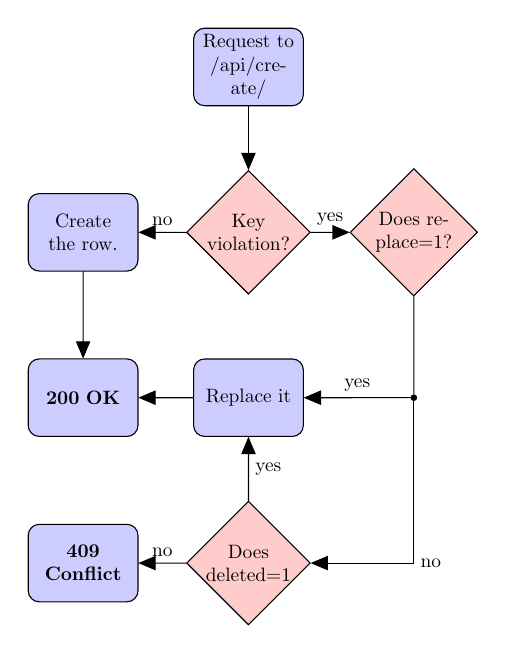
\begin{tikzpicture}[node distance = 3cm, auto, scale=.7, every node/.style={transform shape} ]
  % Place nodes
  \node [block] (request) {Request to /api/create/};
  \node [decision, below of=request] (isconflict) {Key violation?};
  
  \node [block, left of=isconflict] (create) {Create the row.};
  \node [decision, right of=isconflict] (nocreate) {Does replace=1?};
 
  \node [block, below of=create] (ok) {\textbf{200 OK}}; 

  \node [dot, below of=nocreate] (nocreateDOT) {};

  \node [block, left of=nocreateDOT] (replace) {Replace it};
  \node [decision, below of=replace] (isreplace) {Does deleted=1};

  \node [block, left of=isreplace] (error) {\textbf{409 Conflict}};

  % Draw edges
  \path [line] (request) -- (isconflict);
  \path [line] (isconflict) -- node [above] {no} (create);
  \path [line] (isconflict) -- node [above] {yes} (nocreate);
  \path [line] (create) -- (ok);

  \path [edge] (nocreate) -- (nocreateDOT);
  \path [line] (nocreateDOT) -- node [above] {yes} (replace);
  \path [line] (replace) -- (ok);

  \path [line] (nocreateDOT) |- node [right] {no} (isreplace);
  \path [line] (isreplace) -- node [right] {yes} (replace);

  \path [line] (isreplace) -- node [above] {no} (error);

\end{tikzpicture}
\caption{The actions that the server takes for every request to \create that it
receives from clients. This actions depend on clients sending a \term{replaced}
parameter with their requests.}
\label{fig:create}
\end{figure}

The flow chart starts with ``Request to /api/create/'', which is a request
to create a row on the server from a client. If there is no key constraint
violation, then the row is created and the server responds with a \texttt{200
OK}. If there is a violation then the server checks to see if the request's
\texttt{replace} parameter is set to \texttt{1}. If it is then the conflicting
row can be replaced without worry and the server responds with a \texttt{200
OK}.  If not then the server checks to see if the conflicting row is marked as
deleted. If it is, then the conflicting row can be replaced and the server
responds with a \texttt{200 OK}. If not, then the server responds with a
\texttt{409 CONFLICT} and the row is not created. At this point, the client has
enough information to ask the user if they wish to replace (or update) the
conflicting row on the server and potentially resend the request with
\texttt{replace=1}. 
 
This solution reduces the functional burden of the deleted rows, enables SQL
\texttt{UPDATE} functionality, is completely representable with pure SQL, and
requires no significant changes to the existing API. 



In summary, we have created a method of synchronization that utilizes
only standard SQL features and doesn't introduce any dependencies into Coexist. So far,
we have solved the problem of database synchronization and the implementation of
\sync, but have yet to address
the other questions presented in Section~\ref{sec:api}: what will the data
exchange format between the server and clients be, and how will clients know how
to present database contents to the user? However, we have made two important
discoveries about the client: requests to \create must include a
\term{replace} parameter and requests to \sync must include one \var{mod\_ts}
parameter per SQL table. This information will be factored into the design of
the client-server communication model in Section~\ref{sec:communication}





%--------------------------------------------------------
\section{Client-Server Communication} \label{sec:communication}
%--------------------------------------------------------



%Many mobile applications are supplemented by a local database (typically
%SQLite). Some applications are stand alone and use these databases primarily as
%persistent storage; the Networkmaine inventory application uses its local
%database to interface with the remote back end MySQL server that it depends
%heavily on. There were three methods for this interfacing that represent
%different degrees of caching, from none, to selective, to complete.


%Before deciding upon a

This section will explore some of the methods that the client can use to
interface with the server, their advantages and disadvantages, and explain why
the method labeled as the \textit{mirror method} is the appropriate choice. The
following subsections will give details on the implementation of this method and
its implications on the database schema; particularly, how normalized it should
be and how to handle deletions. In all diagrams in this section, the arrows
indicate the flow of data and the labels indicate the actions that cause them.


%-------------------------------------------------------
\subsubsection{Window method}

In the window method, the data that a user sees at any given time is a window
into the back end server; all of the data came from the server and none of it is
going to persist beyond this screen. The major advantage to this method is its
ease of implementation. This would be a suitable fit for a small weather
application; in fact, it is the approach that my own weather application ,
QtWeather, uses.  

%TODO add some more analysis details

\begin{figure}[h!]
\centering
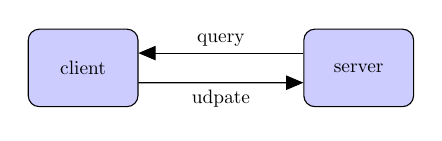
\begin{tikzpicture}[node distance = 2cm, auto, scale=.7, every node/.style={transform shape}]
  % Place nodes
  \node [block] (client) {client};
  \node [block, right of=client, node distance=5cm] (server) {server};
  % Draw edges
  \path [line] (server.165) -- node [above] {query} (client.15);
  \path [line] (client.345) -- node [below] {udpate} (server.195);
\end{tikzpicture}
\caption{Window method}
\label{fig:window}
\end{figure}


%-------------------------------------------------------
\subsubsection{Cache method}

Treating the client as a window requires that we don't have large amounts of
data constantly being retrieved from the server. If this is not the case, then
we may want to identify some data (or queries) that are commonly used in order
to cache (and optionally sync) on the client's local database. This would be
suitable for a mobile social networking client. Take a typical Facebook
application for example; it would be advantageous to cache a users top five
commonly used groups as well as their friend list because this information is
supposedly accessed often and is relatively static. In contrast, caching the
Facebook news feed would probably result in a lot of wasted space because of how
fast it changes and how rarely old news feed entries are viewed. 



\begin{figure}[h!]
\centering
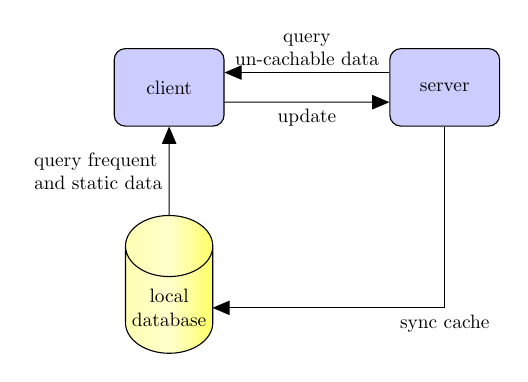
\begin{tikzpicture}[node distance = 2cm, auto, scale=.7, every node/.style={transform shape}]
  % Place nodes
  \node [block] (client) {client};
  \node [block, right of=client, node distance=5cm] (server) {server};
  \node [db, below of=client, node distance=4cm, align=center] (database) {local \\ database};

  % Draw edges
  % Need to align in order to line break
  \path [line] (server.165) -- node [above, align=center] {query \\ un-cachable data} (client.15);
  \path [line] (client.345) -- node [below] {update} (server.195);
  \path [line] (server) |- node {sync cache} (database);
  \path [line] (database) -- node [align=left] {query frequent \\ and static data} (client);
\end{tikzpicture}
\caption{Cache method}
\label{fig:cache}
\end{figure}


%-------------------------------------------------------
\subsubsection{Mirror method}
The window method has the client retrieve all data from the server all of the
time, the cache method identifies some useful data to store and then caches it
locally; the mirror method is the next natural step in this progression: cache
the entire database. There are some immediate concerns with this approach, most
prominent of which concerns the size of the database potentially being much
larger than the what we can reasonably expect to store on the client. The
advantages to this method are faster query times and less reliance on the
network. In fact, this is the only method that would enable a fully readable
database off line.

\begin{figure}[h!]
\centering
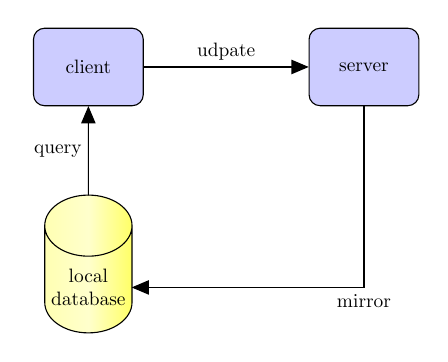
\begin{tikzpicture}[node distance = 2cm, auto, scale=.7, every node/.style={transform shape}]
  % Place nodes
  \node [block] (client) {client};
  \node [block, right of=client, node distance=5cm] (server) {server};
  \node [db, below of=client, node distance=4cm, align=center] (database) {local \\ database};

  % Draw edges
  % Need to align in order to line break
  \path [line] (client) -- node {udpate} (server);
  \path [line] (server) |- node {mirror} (database);
  \path [line] (database) -- node [align=left] {query} (client);
\end{tikzpicture}
\caption{Mirror method}
\label{fig:mirror}
\end{figure}

The Networkmaine inventory database contains information for approximately six
thousand devices, location, purchase order and rma information for batches of
devices; the size of the MySQL database dump is 1.5 megabytes. In addition, the
database will not grow quickly. The size of the database makes the mirror method
very attractive: if Networkmaine added two thousand units a year to its
deployment then in twenty years the size of the database would be no less than
12 megabytes; still reasonable to store on the mobile clients we see available
today (probably more so on the mobile clients in twenty years, if we still use
them). Realistically, there won't be more than a few hundred devices added to
the inventory each year, at most. It is for these reasons that the mirror method
is preferable for this project. 





%--------------------------------------------------------
%\subsection{Database Replication} \label{sec:db}


It is important to ensure that the client can never update the server if the
client is out of sync, and the client must always have a way of re-syncing
itself.  This can be achieved with two simple API functions, \texttt{/api/sync}
and \texttt{/api/schema}; where one function requests missing information and
another requests schema information. This design accounts for the database
schema being upgraded on the server, and clients attempting to make changes to
the database server when out of sync. Figure~\ref{fig:protocol} depicts the
network dialog between a client and server where the client attempts to sync
itself when it is using and old version of the database. 




\begin{figure}[h!]
\centering
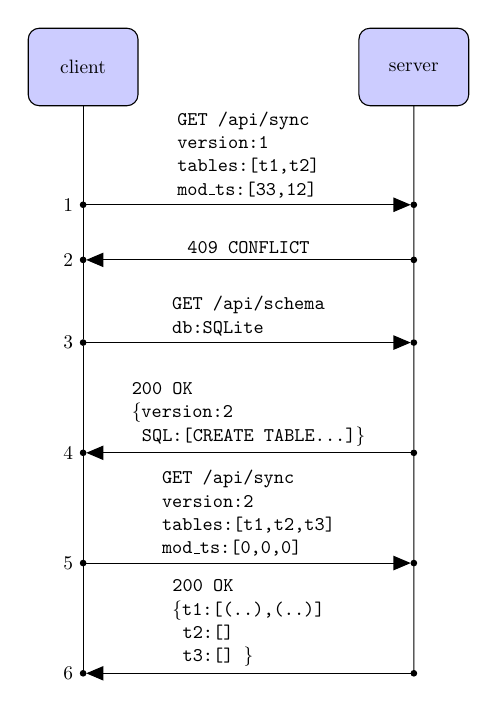
\begin{tikzpicture}[node distance = 2cm, auto, scale=.7, every node/.style={transform shape}]
  % Place nodes
  \node [block] (client) {client};
  \node [block, right of=client, node distance=6cm] (server) {server};
  
  \node [dot, below of=client, node distance=2.5cm, label=180:1] (c1) {};
  \node [dot, below of=server, node distance=2.5cm] (s1) {};
  \path [line] (c1) -- node [above, align=left] {
    \tt\textbf{GET /api/sync} \\ 
    \tt version:1 \\ 
    \tt tables:[t1,t2] \\ 
    \tt mod\_ts:[33,12]}   (s1);
  \path [edge] (client) -- (c1);
  \path [edge] (server) -- (s1);

  \node [dot, below of=c1, node distance=1cm, label=180:2] (c2) {};
  \node [dot, below of=s1, node distance=1cm] (s2) {};
  \path [line] (s2) -- node [above] {\tt\textbf{409 CONFLICT}} (c2);
  \path [edge] (c2) -- (c1);
  \path [edge] (s2) -- (s1);

  \node [dot, below of=c2, node distance=1.5cm, label=180:3] (c3) {};
  \node [dot, below of=s2, node distance=1.5cm] (s3) {};
  \path [line] (c3) -- node [above, align=left] {
    \tt\textbf{GET /api/schema} \\ 
    \tt db:SQLite            } (s3);
  \path [edge] (c2) -- (c3);
  \path [edge] (s2) -- (s3);

  \node [dot, below of=c3, node distance=2cm, label=180:4] (c4) {};
  \node [dot, below of=s3, node distance=2cm] (s4) {};
  \path [line] (s4) -- node [above, align=left] {
    \tt\textbf{200 OK} \\
    \tt\{version:2 \\
    \tt~SQL:[CREATE TABLE...]\} } (c4);
  \path [edge] (c3) -- (c4);
  \path [edge] (s3) -- (s4);
    
  \node [dot, below of=c4, node distance=2cm, label=180:5] (c5) {};
  \node [dot, below of=s4, node distance=2cm] (s5) {};
  \path [line] (c5) -- node [above, align=left] {
    \tt\textbf{GET /api/sync} \\ 
    \tt version:2 \\ 
    \tt tables:[t1,t2,t3] \\ 
    \tt mod\_ts:[0,0,0]}   (s5);

  \path [edge] (c5) -- (c4);
  \path [edge] (s4) -- (s5);


  \node [dot, below of=c5, node distance=2cm, label=180:6] (c6) {};
  \node [dot, below of=s5, node distance=2cm] (s6) {};
  \path [line] (s6) -- node [above, align=left] {
    \tt\textbf{200 OK} \\
    \tt \{t1:[(..),(..)] \\
    \tt~t2:[] \\
    \tt~t3:[] \}} (c6);
  \path [edge] (c6) -- (c5);
  \path [edge] (s6) -- (s5);

\end{tikzpicture}
\caption{Synchronization protocol}
\label{fig:protocol}
\end{figure}

The actions can be described as follows. 

\begin{enumerate}

\item The client sends a GET request to /api/sync on the server, including the database version it is using, an array of table names and an array of maximum modification timestamps for those tables (found in a metacolumn).

\item The server responds with a 409 error message because it is currently using version 2 of the database, while the client is using version 1.

\item The client sends a GET request to /api/schema on the server to get the current schema that the server side database is using. It requests the SQL in SQLite syntax.

\item The server responds with a 200 OK code. The body of the response is a JSON object containing the version of the server's database and the SQL statements that need to be executed in SQLite to build it. The constraints do not need to be sent to the client, only the table declarations (and possibly views). Since the client never updates its own database through SQL, the constraints are not necessary. 

\item The client now has enough information to re-create its database. Since there is nothing on the client that isn't also on the server, the client can simply replace the contents of its database with this new schema. A call to /api/sync is repeated with the new schema. 

\item There is no version conflict; the server responds with a 200 OK code. The body of the response is a JSON object that maps table names to arrays containing all of the tuples that the client is missing. 

\end{enumerate}


The dialog would look slightly different for an out of sync client attempting to
make server changes. In figure~\ref{fig:protocol}, the client supplies the
server with all of the tables and their most recent update timestamps. If the
client was to send this information with each API request then the server could
similarly notify the client when they appear out of date; but timestamps and
table names can be verbose, it would better to send a representative checksum in
their place. Figure~\ref{fig:signature} represents the sha1 checksum that can be
sent in API requests as a \textit{signature} to validate the client; $T$
represents the concatenation of all table names, and $M$ represents the
concatenation of all maximum modification timestamps. The first timestamp should
correspond to the first table, and so on.

\begin{figure}[h!]
\[
sha1(version + T + M + username + sha1(password))
\]
\caption{API request signature.}
\label{fig:signature}
\end{figure}

So for a schema that consisted of the tables $Students$ and $Courses$, with
maximum modification timestamps of $2012-12-01 16:18:31$ and
$2012-12-01 16:18:43$ respectively, under version $1$ of the database, with a
user name of $tim$ and a password of $password$, the signature would be
equal to \hbox{$9d64e5fbba865b491adeeeead91666df8d7cb1ec$}.

%TODO recalculate checksum

%begin{figure}[h!]
%sha1("1StudentsCourses2012-12-01 16:\\
%8:312012-12-01 16:18:43timn5baa6\\
%e4c9b93f3f0682250b6cf8331b7ee68fd8") \\
% 9d64e5fbba865b491adeeeead91666df8d7cb1ec$
%caption{My Listing}
%label{fig:list}
%end{figure}




%--------------------------------------------------------
\section{Designing a Metamodel} \label{sec:metamodel}
%--------------------------------------------------------


%--------------------------------------------------------
\subsection{XML Meta Model}  \label{sec:xml}

A \textit{meta model} is a model of a meta data. Giulieri defined the meta data
(in this context) as ``the meaningful information necessary to fully describe
the UI and database mapping''. In this section, we analyze a representative
sample of one of Evolutility's XML meta models and explain the perceived
reasoning behind its design. Understanding this XML meta model will make the
design of the JSON version in Section~\ref{sec:json} clearer.
Figure~\ref{fig:xml} contains the XML meta model sample.

\begin{figure}[h!]
\centering

\begin{lstlisting}[language=XML]
<?xml version="1.0" encoding="UTF-8"?>
<form label="To Do"  
      xmlns="http://www.evolutility.com">
  <data entity="task" entities="tasks" 
        icon="m-todo.gif" dbtable="EVOL_ToDo" 
        dborder="PriorityID, duedate" />
  <panel label="Task" width="62" >
    <field type="text" label="Title" 
      dbcolumn="title"
      required="1" cssclass="fieldmain" 
      maxlength="255" width="100" 
      search="1" searchlist="1" searchadv="1" />
    <field type="date" label="Due Date" 
      dbcolumn="duedate" 
      maxlength="10" width="40" 
      search="1" searchlist="1" searchadv="1" />
  </panel>
</form> 
\end{lstlisting}
\caption{Sample Evolutility XML meta model}
\label{fig:xml}
\end{figure}

Looking at the XML model it is obvious that the structure is designed around the
user interface. This is noteworthy because the typical approach to
relational-database-backed applications is encumbered by the object-relational
impedance mismatch. When representing data in an object oriented language, one
must agree upon a mapping from the relational database. Technologies like the
Java Persistence API have attempted to solve this problem by allowing
programmers to implicitly specify an object mapping when creating objects in
code\cite{oracle_java_????}, but the approach presented in this section
effectively side steps the issue by mapping the database directly to UI forms,
where an obvious mapping \textit{does} exist.

With this in mind, it becomes easier to understand the semantics of the model.
The root element is a \texttt{form}, inside of which are \texttt{data} and
\texttt{panel} nodes. This information represents the structure of a \textit{ui
form}, or a section of a graphical user interface that is dedicated to user
input (like any paper form you may have encountered). The \texttt{field} nodes
are the nodes that model the actual data in the database. These are grouped
under \texttt{panel}s to represent sections of the UI, implemented, perhaps,
using tabs. Each \texttt{field} contains attributes that specify certain
database related attributes. A full list of attributes can be found on the
original Evolutility submission page\cite{giulieri_minimalist_2011}.

\begin{itemize}
\item \textbf{\texttt{dbcolumn}}: The name of the column that this field represents. The name of the table is given in the \texttt{data} node. Each form ultimately models a table in the database.
\item \textbf{\texttt{label}}: A string that will represent this field in the UI.
\item \textbf{\texttt{type}}: The type of this field. Field types are not analogous with database types.
\item \textbf{\texttt{maxlength}}: Some UI metadata to allow visual customization. 
\item \textbf{\texttt{width}}: Similar to maxlength.
\item \textbf{\texttt{search}}: Specifies whether or not this field should appear in a search form. This allows users to hide fields that get auto populated from triggers.
\end{itemize}

Using this model, Evolutility generates Web UI forms at run time. This means
that no code has to be written for the developer to configure and change the
applications functionality and appearance. 

The distinction between form types and database types is a flexible concept that
enables additional UI functionality without jeopardizing the mapping between the
database and UI. 

\begin{figure}[h!]
\centering
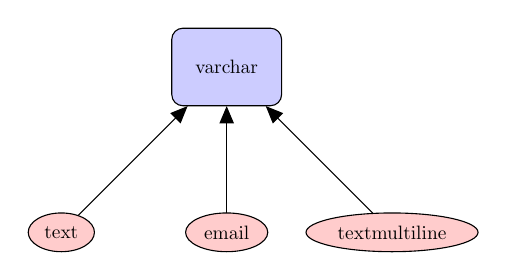
\begin{tikzpicture}[node distance = 2.5cm, auto, scale=.7, every node/.style={transform shape}]
  % Place nodes
  \node [block] (varchar) {varchar};
  \node [cloud, below of=varchar] (email) {email};
  \node [cloud, left of=email] (text) {text};
  \node [cloud, right of=email] (textm) {textmultiline};
  % Draw edges
  \path[line] (email) -- (varchar);
  \path[line] (text) -- (varchar);
  \path[line] (textm) -- (varchar);

\end{tikzpicture}
\caption{UI forms that map to the SQL \texttt{varchar} type.}
\label{fig:varchar_map}
\end{figure}

Figure~\ref{fig:varchar_map} shows the general relationship between UI types
(shown in red) and SQL types (shown in blue). There are generally a number of UI
types that map to a single database type. The difference between any two UI
types that map to the same database type lie in their functionality. For
example, the \texttt{text} UI type will cause fields to be presented as a single
line of text, the \texttt{textmultiline} type will cause a fields to appear as
text boxes, and the \texttt{email} type will cause fields to appear as a single
line of text and enforce email style validation. 




%--------------------------------------------------------
\subsection{JSON Metamodel} \label{sec:json}

%In this section, we examine the shortcomings of Evolutility and introduce a JSON
%model that is equivalent to the XML model of Section~\ref{sec:xml}. 
%
%
%
%\begin{figure}[h!]
%\begin{lstlisting}[language=json]
%{
%  "forms" : [
%  {
%    "label":"RMA",
%    "table":"RMA",
%    "fields": [
%      {"label":"RMA Number","type":"barcode",
%         "column":"rma_no"},
%      {"label":"Sent","type":"date",
%         "column":"sent"},
%      {"label":"Returned","type":"text",
%         "column":"returned"},
%      {"label":"Note","type":"text",
%         "column":"note"},
%      {"label":"Serial","type":"reference",
%       "column":"serial_no","required":true,
%       "references":{
%         "table":"Devices",
%         "column":"serial_no"
%    }}
%    ]
%  }
%  ]
%}
%\end{lstlisting}
%\caption{Sample JSON meta model.}
%\label{fig:json_sample}
%\end{figure}
%
%The general form of the model is similar Evolutility's XML version. The first
%attribute in the object is \texttt{form}, which references an array of forms.
%Each form contains attributes that specify the database-UI mapping and UI
%metadata. The \texttt{label} and \texttt{table} of forms represent the title and
%the database table that it models, and the \texttt{fields} array contains
%\texttt{field} objects that model the actual data. The approach to
%\texttt{fields} has been altered and expanded. In the XML model, a foreign key
%was modeled as \texttt{lov} type (list of values). It would use integer primary
%keys to identify valid values in other tables. In Coexist, that type has been
%changed to the \texttt{reference} type, and an additional \texttt{references}
%attribute has been added to model the foreign key relationship, relieving the
%integer primary key requirement. In Figure~\ref{fig:json_sample}, the column
%\texttt{serial\_no} of table \texttt{RMA} is a foreign key on the
%\texttt{serial\_no} column in the \texttt{Devices} table. 
%
%Since Coexist was designed with mobile clients in mind, there have been several
%UI types added to take advantage of smart phone functionality. The
%\texttt{barcode} type is the same as a \texttt{text} type, except it causes a
%barcode to appear on the right of it, allowing users to get input from a barcode
%using a smart phone's camera. The \texttt{image} type has been updated from
%Evolutility in this same fashion; it now presents a camera icon that allows
%users to receive input from a camera, ultimately mapping to a SQL \texttt{blob}
%type. The \texttt{location} data type allows users to use GPS as input, storing
%latitude and longitude information as a SQL \texttt{varchar} type.



%%%%%
% GOAL: be able to write metamodels by hand, being aware of all features


% before here, declare what the metamodel has to represent, and why it has 
% things like 'label' and 'table' etc.


Section~\ref{sec:replication} defined the synchronization process between the
server and clients and introduced some requirements for the communication
protocol. This section focuses on modeling the mapping of database information onto the
user interface. Specifically, this section will introduce a \textit{metamodel}
that contains all of the information that any Coexist client needs in order to
display the database contents to users. A metamodel is simply a model that deals
with \textit{metadata}, where metadata is any data about the application itself.


Without knowing any specific details about the application, we know that there
will be screens dedicated to user-data-entry. Figure~\ref{fig:sample_form}
contains a form that will appear (at least conceptually) in Coexist.

\begin{figure}[h!]
\center
\begin{tabular}{r l}
  Your name: &  \underline{\makebox[1in][1]{}}   \\
  Exercise: &  \underline{\makebox[1in][1]{}}   \\
  Weight: &  \underline{\makebox[1in][1]{}}   \\
  Date: &  \underline{\makebox[1in][1]{}}   \\
\end{tabular}
\caption{A form that is used for data entry. This simple example can be analyzed
to determine what the client needs to know about the data it handles in order to
display this form to users.}
\label{fig:sample_form}
\end{figure}

In this example, the database in question tracks statistics for workouts. The
form in Figure~\ref{fig:sample_form} allows a user to input their name, an
exercise, a weight and a date into the database. If forms of this type are going
to appear in Coexist, then clients will have to know
\begin{inparaenum}
\item what table this data should be inserted into,
\item what data goes in each column, and
\item how to filter input.
\end{inparaenum}
Figure~\ref{fig:sample_table} contains the SQL that creates the database table
that this form will upload to, without any consideration for the form's layout.

\begin{figure}[h!]
\begin{lstlisting}[language=sql]
CREATE TABLE workout_log(
  user VARCHAR(10),
  exercise VARCHAR(10) REFERENCES Exercises,
  weight INTEGER,
  date_done DATE);
\end{lstlisting}
\caption{A SQL database that tracks workout information. The form in
Figure~\ref{fig:sample_form} will be used to upload data into this table.}
\label{fig:sample_table}
\end{figure}

The ordering of the fields in the form correspond to the ordering of the columns
in the table (in this example), but the names presented in the form differ from
the column names. With this, we can start defining the contents of the Coexist
metamodel. Figure~\ref{fig:json_form} contains the JSON that will be used for
representing forms in the metamodel.

\begin{figure}[h!]
\begin{lstlisting}[language=json]
{
  "forms" : [
  {
    "label":"Workout",
    "table":"workout_log",
    "fields": [...]
  }
  ]
}
\end{lstlisting}
\caption{A sample metamodel featuring the \texttt{forms} attribute. The
\texttt{forms} attribute represents a single UI mapping for a SQL table.}
\label{fig:json_form}
\end{figure}

It's worth saying that JSON can easily be replaced with YAML or XML, as other
similar projects have done\cite{giulieri_minimalist_2011}. Coexist supports JSON
primarily, but there is nothing in the code base that specifically depends on
data being JSON -- alternative languages can be added in the future.

In Coexist, a \texttt{form} encapsulates a database table. In
Figure~\ref{fig:json_form}, the \var{forms} attribute contains an array of
\var{form} objects (only one in this case). The \var{form} object with a
\var{label} of \var{Workout} represents the database table in
Figure~\ref{fig:sample_table} and enables the form in
Figure~\ref{fig:sample_form} to display more readable names in the user
interface. The \var{fields} attribute contains an array of \var{field} objects,
which represent individual fields in forms, like the ``Name'' field in the form
of Figure~\ref{fig:sample_form}, and ultimately correspond to columns in
database tables. Figure~\ref{fig:json_field} contains the \var{field} objects that
are hidden behind the \var{\ldots} in Figure~\ref{fig:json_form}.


\begin{figure}[h!]
\begin{lstlisting}[language=json]
{
  "label":"Your name"
  "column":"user"
  "type":"string"
},
{
  "label":"Exercise"
  "column":"exercise"
  "type":"reference"
  "references":
  {
    "table":"Exercises"
    "column":"exercise"
  }

},...
\end{lstlisting}
\caption{A sample metamodel featuring the \texttt{field} object. Each
  \texttt{field} object represents a single UI mapping for a column in a SQL
table.}
\label{fig:json_field}
\end{figure}

Figure~\ref{fig:json_field} shows the UI mapping for the table's columns, where
each JSON object is a \textit{field}. The first field enables the client to
present the \var{user} column as ``Your name'' in the form. The most important
take-away from this model is the typing system, allowing the client
to filter input from users. In this example, the type of the \var{user} field is
\var{string}, which means that it accepts any string. The type of the
\var{exercise} field is \var{reference}, which is how foreign keys are modeled
in the Coexist metamodel. With forms and fields, Coexist clients can effectively
map the contents of the database onto the user interface. The next section will
define all of the types available in the Coexist metamodel.


%--------------------------------------------------------
\subsection{Metamodel types}  \label{sec:types}

Having types isn't strictly necessary -- it is possible to have clients only
display labels and entry fields and have the server reject invalid input if
it gets uploaded. Having types allows Coexist to leverage the features of
different client types effectively. For example, Coexist supports a
\var{barcode} type that allows clients on supporting platforms to read barcodes
with cameras. This section will continue to define metamodel types that Coexist
clients can use to filter user input. There are four disjoint types from which
all types inherit: \var{string}, \var{numeric}, \var{blob} and \var{reference}.
In most cases, when a subtype inherits from a parent type, the subtype may only
offer a data input hint.


%--------------------------------------------------------
\subsubsection{String types}  \label{sec:type_string}
Fields of type \var{string} can take any string as their input. They correspond
roughly to the \var{varchar} SQL type (and other types like \var{text} in different SQL
implementations). There are also several types that inherit from \var{string}.
The \var{barcode} type is treated as a string as far as a relational database is
concerned, but the Coexist client will allow users to scan barcodes when
entering data instead of having to use the keyboard. The \var{email} type is
also a subtype of \var{string}, where clients have the opportunity to validate
input as an email address before allowing requests to leave. The \var{date} and
\var{timestamp} types also inherit from \var{string}, allowing clients to
present appropriate dialogs for data entry.



%--------------------------------------------------------
\subsubsection{Numeric types}  \label{sec:type_num}

The \var{numeric} type is the base type for all numbers in Coexist. From this
type, the \var{integer} type inherits. Any data sent to the server is ultimately
sent as a string, so the differences between these types is purely cosmetic:
\var{numeric} allows numbers in $\mathbb{R}$, and \var{integer} allows numbers in
$\mathbb{Z}$. 


%--------------------------------------------------------
\subsubsection{Blob types}  \label{sec:type_blob}

Fields of type \var{blob} store some kind of blob data. The default input method
for these types is to select a file from the file system that gets dumped into
the request. For subtypes like \var{photo}, clients on supporting platforms can
launch camera applications to take pictures and send them in requests.


%--------------------------------------------------------
\subsubsection{The reference type}  \label{sec:type_reference}

The \var{reference} type is unique in that it has no subtypes. It is used to
model foreign keys in the database. It is used in Figure~\ref{fig:json_field} by
first declaring a type of \var{reference} and then by defining a
\var{references} property to let clients know which table and column the column
in question is dependent on. The \var{reference} type is a hint to clients that
the value for their field should be selected from a list of values --
specifically a list of unique attributes in the table that is referenced.

Using only the \var{field} and \var{form} JSON objects shown in
Figures~\ref{fig:json_form} and \ref{fig:json_field}, a metamodel can be
constructed that allows Coexist clients to effectively display and collect data
to and from users. Next, we consider how developers using Coexist will create
and maintain metamodels.


%--------------------------------------------------------
%\newcommand{\sql}[1]{\texttt{#1\textsubscript{sql}}}
%\newcommand{\mm}[1]{\texttt{#1\textsubscript{mm}}}
\newcommand{\sql}[1]{\texttt{$#1_{sql}$}}
\newcommand{\mm}[1]{\texttt{$#1_{mm}$}}
\subsection{Creating individual metamodels}  \label{sec:}

Having a JSON metamodel solves the problem of mapping database information onto
the user interface, but it introduces a new component that users will have some
responsibility for maintaining. Crafting small metamodels by hand is at best
time-consuming, becoming increasingly daunting as the size of database
schemas increase.  This section will introduce a program, \term{modelgen} (metamodel
generator), that mitigates this overhead for users, and discuss the reasoning
for its design.

Since the metamodel encapsulates the database schema, \term{modelgen} can either take
a metamodel and map it to SQL, or vice versa. Before choosing, we must
understand the actual mapping between the Coexist JSON metamodel and SQL,
starting with mapping SQL to the metamodel. Figure~\ref{fig:metamodel_sql}
contains three sample of semantically equivalent SQL. The first and second
samples are typical of how a human would write SQL, while the third is more
likely to come from tools like mysqldump. None the less, there is no guarantee
about which sample \term{modelgen} will be asked to convert.

\begin{figure}[h!]
\begin{lstlisting}[language=sql]
-- First sample
CREATE TABLE Enrolled (
  id INTEGER REFERENCES Students(id));

-- Second sample
CREATE TABLE Enrolled (
  id INTEGER
  CONSTRAINT fk FOREIGN KEY REFERENCES Students(id));

-- Third sample
CREATE TABLE Enrolled ( id INTEGER );
ALTER TABLE Enrolled
  ADD CONSTRAINT fk FOREIGN KEY (id) REFERENCES Students;
\end{lstlisting}
\caption{Three samples of SQL that are semantically equivalent. They will need
to be represented in the metamodel as JSON.}
\label{fig:metamodel_sql}
\end{figure}

The equivalence of these three SQL samples implies that \term{modelgen} would be a
many-to-one function if it took SQL and produced a metamodel.
Figure~\ref{fig:metamodel_json_convert1} shows the relevant portion of the
metamodel that would represent each of the three SQL samples equally.
Designing \term{modelgen} to take SQL and produce a metamodel poses several problems.

\begin{figure}[h!]
\begin{lstlisting}[language=json]
{
  "label":"Enrolled",
  "table":"Enrolled",
  "fields": [
    {"label":"Serial",
     "column":"serial_no",
     "type":"reference",
     "references":{
       "table":"Students",
       "column":"id"}}
  ]
}
\end{lstlisting}
\caption{A single field in the metamodel that equally represents all three
samples in Figure~\ref{fig:metamodel_sql}.}
\label{fig:metamodel_json_convert1}
\end{figure}


%\subsubsection{$f : type_{SQL} \rightarrow type_{metamodel}$ is not surjective}
\subsubsection{Mapping SQL types to metamodel types is not surjective}
\label{sec:metamodel_issue1}

The mapping from SQL syntax to metamodel syntax is surjective, but the
mapping from SQL types to metamodel types is not. For example, \var{id} in
Figure~\ref{fig:metamodel_sql} is an integer, but the metamodel defines
integer, and barcode, the latter of which is essentially an
integer, but allows clients to present a barcode scanner for user input (if
they support it). This means that \var{modelgen} would have to default the conversion
from SQL integer to an integer, and it would never produce a metamodel with
a barcode in it. A similar situation occurs when converting a
varchar; it can be represented as a text, email, or textbox.


%--------------------------------------------------------
\subsubsection{Metamodels represent more than SQL}  \label{sec:}

%If there are two functions, $f$ and $g$, and a metamodel, $M1$, then
%\[
%f : SQL \rightarrow metamodel
%\]
%\[
%g: metamodel \rightarrow SQL
%\]
%\[
%f(g(M1)) \neq M1
%\]

Given a function $(f:SQL \rightarrow metamodel)$ and \mbox{$(g:metamodel
\rightarrow SQL)$}, and a metamodel $M1$, $f(g(M1)) \neq M1$.
This is because the metamodel contains information that cannot be
represented in SQL, like the \var{label} field, which is used for display
purposes in client applications. Given the metamodel in
Figure~\ref{fig:metamodel_json_convert1}, if we
\begin{inparaenum}
\item change the first \var{label} property to \var{``All enrolled''},
\item convert it into SQL, and
\item convert it back into a metamodel,
\end{inparaenum}
the value of the \var{label} will be lost (defaulted to the value of the table
name), because SQL says nothing about how the data should be displayed in
applications. When converting from SQL, it is likely that a
user will be required to hand edit the metamodel and insert values for fields
like \var{label}.

In summary, the two largest issues with mapping SQL to metamodels is a lossy,
many-to-one syntax-translation and an injective, non-surjective type-translation.
Both of these issues imply that going in the reverse direction is more
favorable. There are a few stipulations, namely that 
\begin{inparaenum} 
\item one of the many possible SQL translations needs to be chosen and
\item the metamodel has to be able to represent some database related information
like primary and foreign keys.
\end{inparaenum}

Much like in Figure~\ref{fig:metamodel_sql}, we only consider different SQL
options that are semantically equivalent to each other and accurately represent
the metamodel being translated. Specifying that the SQL under consideration must
be equivalent with each other is important because it is possible to have two
different SQL statements that represent the same metamodel, but are not
technically equivalent with each other. For example, adding \var{ENGINE=InnoDB}
to sample 1 from Figure~\ref{fig:metamodel_sql} has implications on the
database, but it wouldn't change the semantics of the SQL as far as the
metamodel is concerned. To deal with this, we will only consider minimal SQL
samples, or samples of SQL that are all equivalent and don't have any additional
non-semantic parts. This usually means that we will disregard DBMS specific
features.

Since we only consider semantically equivalent SQL, any SQL chosen will work.
As a sort of tie-breaker, the SQL that makes the user's experience more
convenient will be selected. Of the three samples in Figure~\ref{fig:metamodel_sql},
sample 1 is the most simple. However, sample 2 has a significant functional advantage
over sample 1: its foreign key can be deleted because it has a name. So of the
three samples, sample 2 seems to be the best choice, and a similar reasoning
will be applied to other cases. There are several advantages to mapping
metamodels to SQL as well. Specifically, mapping in this direction allows
Coexist to do two things.


%--------------------------------------------------------
\setcounter{subsubsection}{0}
\subsubsection{Handle clients of any DBMS} \label{sec:mm_advantage}

Originally, users would have to create SQL schemas for every type of DBMS that
they intended to use on clients. If a user chose MySQL for the central server's
DBMS, and only Android clients were going to be used, then that user would have
to store a SQLite compatible version of the MySQL schema on the server so that
clients could build a local version of the central database.

If \term{modelgen} can generate schemas from metamodels then users no longer have to
store copies of SQL schemas in different DBMS-compatible forms for
clients. Figure~\ref{fig:modelgen_flow} depicts the dialog between a coexist
client and server, where the client requests the schema it should use for its
local storage.


\begin{figure}[h!]
\centering
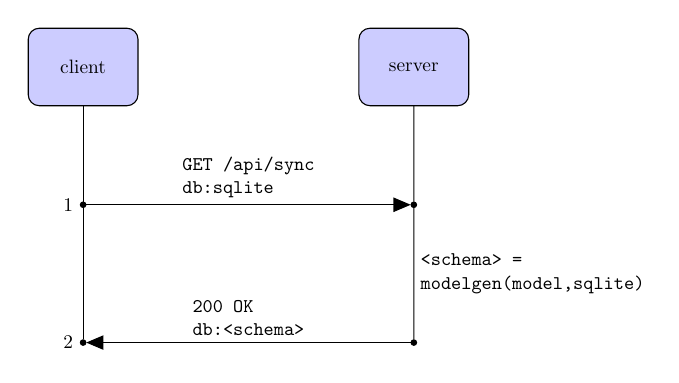
\begin{tikzpicture}[node distance = 2.5cm, auto, scale=.7, every node/.style={transform shape}]
  % Place nodes
  \node [block] (client) {client};
  \node [block, right of=client, node distance=6cm] (server) {server};
  
  \node [dot, below of=client, label=180:1] (c1) {};
  \node [dot, below of=server] (s1) {};

  \node [dot, below of=c1, label=180:2] (c2) {};
  \node [dot, below of=s1] (s2) {};
  

  \path [line] (c1) -- node [above, align=left] {
    \tt\textbf{GET /api/sync} \\ 
    \tt db:sqlite}   (s1);


  \path [line] (s2) -- node [above, align=left] {
    \tt\textbf{200 OK} \\ 
    \tt db:<schema>}   (c2);


  \path [edge]  (client) -- node  {} (c1);
  \path [edge]  (server) -- node  {} (s1);
  
  \path [edge]  (c1) -- node [above] {} (c2);
  \path [edge]  (s1) -- node [right, align=left] {
    \tt  <schema> = \\
    \tt modelgen(model,sqlite)}   (s2);

\end{tikzpicture}
\caption{A dialog between a Coexist client and server where the client requests
the schema it should use for local storage.}
\label{fig:modelgen_flow}
\end{figure}

Figure~\ref{fig:modelgen_flow} starts at step 1, where the client requests the
schema it should be using for its local storage. The server generates the
schema in a SQLite compatible form and returns it to the client in step 2. This
behavior requires no changes to the communication model established in
Section~\ref{sec:communication}.




%--------------------------------------------------------
\subsubsection{Add metacolumns to the schema} \label{sec:mm_advantage}

As discussed in Section~\ref{sec:replication}, database schemas require the
addition of metamodels to enable database replication. If \term{modelgen} is creating
the schemas, then the metacolumns, triggers, and indexes can be automatically
added. Figure~\ref{fig:modelgen_save} shows the non-trivial amount of SQL
boilerplate that users would have to add themselves for \emph{every} table
in their database schema.


\begin{figure}[h!]
\begin{lstlisting}[language=SQL]
-- Adding two metacolumns to tables
CREATE TABLE Name (
  ...,
  mod_ts TIMESTAMP,
  deleted INTEGER);
-- A trigger for UPDATE, INSERT, and REPLACE
CREATE TRIGGER mod_ts AFTER INSERT ON Student
  FOR EACH ROW SET mod_ts = NOW();
-- An index on the commonly searched mod_ts
CREATE INDEX modts_index ON Name (mod_ts DESC);

\end{lstlisting}
\caption{Three types of SQL statements that need to be added to every table in
every schema in Coexist. These statements are automatically added when  users
generate schemas with \term{modelgen}.}
\label{fig:modelgen_save}
\end{figure}


At this point, we have addressed all of the concerns in Section~\ref{sec:api}.
We have defined a pure SQL synchronization algorithm in
Section~\ref{sec:replication}, outlined a communication protocol in
Section~\ref{sec:communication}, and specified a JSON based metamodel that
clients can use to map database contents onto user interfaces in this section.
Next, in Section~\ref{sec:deployment}, we examine the Coexist system as a whole,
from a user's point of view.
%Next, in Section~\ref{sec:api_imp}, we will revisit the API methods declared in
%Section~\ref{sec:api} and finalize their implementation. 






%--------------------------------------------------------
%\section{Implementing the API Methods} \label{sec:api_imp}
%--------------------------------------------------------


%--------------------------------------------------------
\section{Deployment} \label{sec:deployment}
%--------------------------------------------------------



%--------------------------------------------------------
\subsection{coexist.ini file}  \label{sec:ini}


% use relative file paths

\begin{itemize}
\item \bt{name} The name of the application. It will be seen in the main window of the Android application, title of Web pages etc.
\item \bt{image} An image icon for the application. On Android, this will be the icon that users click to launch the application.
\item \bt{notification} An image icon for the application's notifications. This can optionally be the same as the \bt{image} parameter, but most Android applications have a grey scale version of \bt{image} here instead.
\item \bt{package} The unique java style domain for your application. If a particular instance is going to be an inventory application for a company with the domain \bt{domain.com} then this field might be \bt{com.domain.inventory}. This field is important because Android requires all applications to have a unique package name. 
\item \bt{api} The URL of the Coexist server API. If this is the first time Coexist is being configured then the server API would not have been deployed yet, but the location is still required. This field could be \bt{http://domain.com/api/}; this is the URL that the clients will send their requests to. 
\item \bt{version} This is the current version of the application (i.e. 1). This will ultimately reside in a directory of the server API (that gets created using this file) \bt{conf/conf.ini}. If it is ever incremented then it will reject all client requests that are using different versions with a 409 error code and cause them to resync and upgrade. More on this in the server section ??.
\item \bt{user} The user name of the database for the server API's use.
\item \bt{pass} The password of the database for the server API's use.
\item \bt{db} The name of the database for the server API's use.
\item \bt{host} The hostname of the database for the server API's use.
\item \bt{dbms} The database type (i.e. mysql, postgresql) for use in the server API's PHP PDO calls. It should support any database type that the PDO library does.
\item \bt{ui} The location of the ui dir that should be included in the server API. This is explained further in the UI Dir section ??.
\item \bt{sql} The location of the sql dir that should be included in the server API. This is explained further in the SQL Dir section ??.
\item \bt{android} An on/off value can be used to enable or disable the Android build.
\item \bt{Web} An on/off value can be used to enable or disable the server API build.
\item \bt{scp\_to} An experimental key that can be used to better automate the build process. A possible value might be \bt{user@domain.com:/srv/domain.com/}. This would cause the resulting apk and tgz packages to be copied to the target server using scp. The public facing content in the tgz package is in a folder named htdocs, so the sample \texttt{scp\_to} value would be especially wise if the document root was \texttt{/srv/domain.com/htdocs} because a simple un-tar would be all that was required. 
\item \bt{scp\_port} Just in case the ssh server is running on a non standard port.
\end{itemize}





%--------------------------------------------------------
\subsection{Create the database.}  \label{sec:}

ShoppingList is a simple application, consisting of one table called
\texttt{Items}. Create the database and a user on the server, and execute the
SQL to create the desired table and meta data trigger. Its not hard to manually
create the triggers when there are few tables, but it can be tedious as more
tables are added. In \texttt{Web/bin}, there is a script called
\texttt{mktriggers} that will parse SQL files and send triggers to stdout. A
version of this file should also be saved in \texttt{Web/lib/SQL/SQLite/1}.
Saving it in this location means that it will be given to clients that use
Sqlite for version \texttt{1} of the application.


\begin{figure}[h!]
\begin{lstlisting}[language=sql]
REATE TABLE Items(
  item VARCHAR(100),
  mod_ts DATETIME, --metacolumn
  deleted INTEGER, --metacolumn
  CONSTRAINT item_pk PRIMARY KEY (item)
);

CREATE TRIGGER Items_trigger 
  BEFORE UPDATE ON Items 
  FOR EACH ROW SET NEW.mod_ts=NOW();
\end{lstlisting}
\caption{ShoppingList SQL file.}
\label{fig:shoppinglist_SQL}
\end{figure}




%--------------------------------------------------------
\subsection{Create the JSON meta model.}  \label{sec:}

A simple database requires an equally simple JSON meta model. The following
model will create a single \textit{Items} form on the client, consisting of the
\texttt{text field} \textit{Item}. This file should be saved in
\texttt{Web/lib/ui/1/}, for the same reasons as the previous SQL file.

\begin{figure}[h!]
\begin{lstlisting}[language=json]
{
  "forms" : [
  { 
    "label":"Items",
    "table":"Items",
    "fields": [
    {"label":"Item", "type":"text","column":"item"}
    ]
  }
  ]
}
\end{lstlisting}
\caption{ShoppingList JSON meta model.}
\label{fig:shoppinglist_json}
\end{figure}













%--------------------------------------------------------
\subsection{Start the Android application and let it sync.}  \label{sec:}

Once the application is installed and opened, the screen will be blank and spinning. 


\begin{figure}[h!]
\centering

\includegraphics[width=0.25\textwidth]{images/new.png}
\caption{ShoppingList on first launch.}
\label{fig:first_launch}
\end{figure}

In the overflow menu there is an option called \texttt{Sync Now} that will trigger a sync.


\begin{figure}[h!]
\centering

\includegraphics[width=0.25\textwidth]{images/dl.png}
\caption{ShoppingList after first sync.}
\label{fig:first_sync}
\end{figure}

This will cause the client to request the appropriate SQL file and JSON meta
model file from the server. Using this, it will create a local version of the
database and request all missing rows (which will be all rows). It will finish
by reporting the total amount of rows that it received, as seen in
Figure~\ref{fig:first_sync}


%\begin{figure}[h!]
%    \centering
%    \begin{subfigure}[b]{0.1\textwidth}
%        \centering
%        
\includegraphics[width=\textwidth]{images/s1.png}
%        \caption{Home}
%        \label{fig:home}
%    \end{subfigure}%
%    ~ %add desired spacing between images, e. g. ~, \quad, \qquad etc.
%      %(or a blank line to force the subfigure onto a new line)
%    \begin{subfigure}[b]{0.1\textwidth}
%        \centering
%        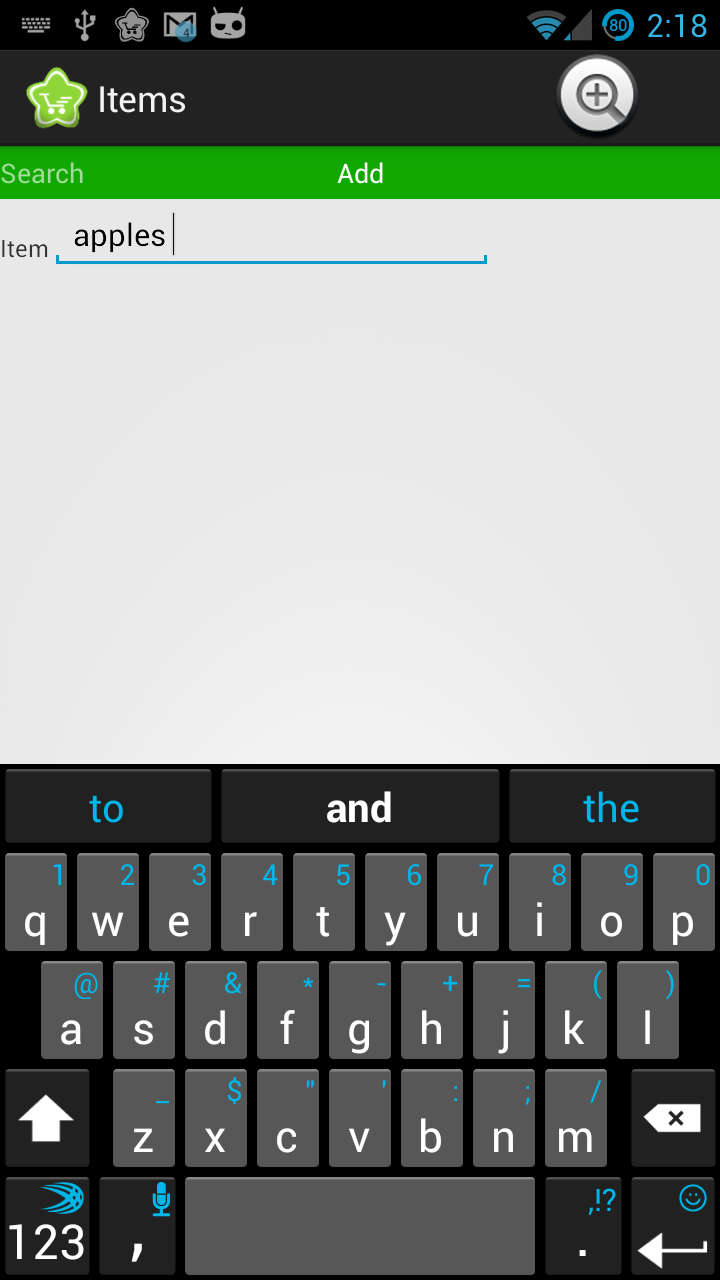
\includegraphics[width=\textwidth]{images/s2.png}
%        \caption{Add}
%        \label{fig:add}
%    \end{subfigure}
%    ~ %add desired spacing between images, e. g. ~, \quad, \qquad etc.
%      %(or a blank line to force the subfigure onto a new line)
%    \begin{subfigure}[b]{0.1\textwidth}
%        \centering
%        
\includegraphics[width=\textwidth]{images/s3.png}
%        \caption{Browse}
%        \label{fig:browse}
%    \end{subfigure}
%    \caption{Final ShoppingList application screens.}\label{fig:shoppinglist}
%\end{figure}


At this point the application is fully functional. Clicking on the
\texttt{Items} section in the home screen will bring launch the CRUD screen for
it. Swiping to the right will reveal the UI form generated by the JSON meta
model and swiping to the left will allow browsing of the database contents. 






%
%%--------------------------------------------------------
%\section{Conclusion} \label{sec:conclusion}
%%--------------------------------------------------------
%
%Much of the setup work can be reduced to simple script execution. In the end,
%Coexist will be configurable through a dedicated tool that pulls down the latest
%stable code from whichever repository it is currently being hosted at and
%automatically configures it based on a name, domain, icon and server
%information.

%tools to auto generate JSON from SQL, or vice versa









%--------------------------------------------------------
%\subsection{Android application structure.}  \label{sec:}
%talk about how flatter is better







%-------------------------------------------------------
% Bibliography
%-------------------------------------------------------
\bibliographystyle{IEEEtran}
\bibliography{report}
\end{document}


